\chapter{入门:矢量与张量}

\extrainfo{“这个理论对所有真正懂它的人产生了深刻的影响;它象征着由Gauss、Riemann、Christoffel、Ricci和Levi-Civita创立的绝对微分学的胜利。”\footnote{Albert Einstein, "Contribution to the Theory of General Relativity", 1915; as quoted andtranslated by C. Lanczos in \href{https://aapt.scitation.org/doi/10.1119/1.9734}{The Einstein Decade}, p. 213.}}


这本小书讲的正是爱因斯坦的点金石---绝对微积分绝对微积分,如今它被称作\textbf{张量分析}。不过,我写这本书时并没有着眼于广义相对论,而是着眼于连续介质力学,这是一种更为简单的理论,它分析“我们每天看到和使用的大量物质:空气、水、土、人体、木头、石头、钢铁、混凝土、玻璃、橡胶……”\footnote{Truesdell and Noll , The Non-Linear Field Theories of Me chanics, p. 1. Two outstanding introductory texts on continuum mechanics are A First Course in Rational Continuum Mechanics, 2nd ed, by Truesdell and Continuum Mechanics by Chadwick.}

连续介质力学虽然是广义相对论的一种极限情况,但是我们在处理它的时候最好是根据它的特点来处理。这样来看的话,两种理论的基础具有本质差别。连续介质力学需用的几何是三维欧几里得空间(简称$E_3$)与一维实轴。而广义相对论需用的几何是四维黎曼流形(球面是二维黎曼流形)。如果你只满足于精通广义相对论(并想参考Misner、Thorne 和 Wheeler 的《万有引力》),看到这里也请振作。在我们即将打造的工具中,我们也可以找到攀登广义相对论顶峰的装备。而那些灌溉了,或者说嵌入,连续介质力学花园的东西本质上是一种弯曲的二维连续体,称作壳,它以不起眼的形式反映了在盛开的广义相对论的花朵中发现的几乎所有数学枝叶。

在试图用数学语言描述力学规律时,我们面临着两个问题。一个是,如果要量化物理现象和对象,就必须引入参考系和该参考系下的坐标系\footnote{所谓参考系,就是用数学的语言来描述物理世界,它给物理世界(\textbf{World},简记作$\mathscr{W} $)中每一个事件(\textbf{Event},简记作$e$)都打上了一个“戳”,这个“戳”的信息包括它在$E_3$中的位置(即空间点)以及它发生的时刻,用实轴$\mathbb{R} $上的一个点表示。换言之,参考系就是从物理世界$\mathscr{W} $到$E_3\times \mathbb{R} $的一个映射$f$。

参考系中的坐标系为每个位置分配一个唯一的三元实数组$n,v,w$,称为空间坐标,并为每个时刻分配一个唯一的数字$t$,称为时间.}。另一个是,由于参考系与坐标系仅仅是脚手架,所以我们无需参考系与坐标系也应当能(以不变的形式)表述物理定律。事实上,这就是广义相对论的宏伟目标。

然而,在连续介质力学中,存在着被称为惯性系的特殊参考系;牛顿的质点运动定律---力等于质量乘以加速度加速度---只在这种参考系下成立\footnote{惯性系也很特殊,但是是另一种不同,而在广义相对论中,参考系是坐标系! (物理学是几何学) 我们可以在广义相对论中引入惯性系,就像我们可以在球体上一点的任意小邻域中引入二维笛卡尔坐标系一样。}。因此,连续介质力学的一个基本关注点是,像牛顿定律这样的定律如何从一个参考系转换为另一个参考系\footnote{改变参考系意味着,如果两个参考系彼此相互运动,同一事件$e$会在两个参考系中投影出不同的$E_3$中的位置$P_1$和$P_2$,以及$\mathbb{R}$上的不同时刻$T_1$和$T_2$。}。除了练习4.24外我们将不分析参考系的转换,相反,我们将探讨一个固定的参考系中,当一个坐标系(例如笛卡尔坐标系)被另一个坐标系(如球坐标系)所取代时,研究对象或是物理定律的数学表达式如何变化。

下文中,我将假设你已经学过一些平面几何以及立体几何的内容,并且假设你已经了解了一些关于矢量代数以及微积分的知识。为了简洁起见,我在探讨时省略了一些细节和例子,你可以参考其他专门介绍矢量的书。同时我也着重强调了几个重点,特别是大部分书中都找不到的,关于矢量加法与分量表示的物理意义。每一章结尾的练习旨在对正文中的内容进行补充和拓展。







\section{三维欧几里得空间}

三维欧几里得空间,$E_3$,可以用一组公理来描述,它表达了被称为点、线等\footnote{这正是希尔伯特的纲领:将几何简化为逻辑的一个分支。不允许有图! (可以参见Eisenhart的《Analytic Geometry》末尾的讨论)然而,我们这本书的方法应该是不拘束并且直观的。}这些原始的、未定义的量之间的关系。这些关系与物理世界中普通的距离测量结果是如此的接近,以至于在广义相对论出现之前,人们认为欧几里得几何就是宇宙的运动学模型。





\section{有向线段}

有向线段或箭头在欧几里德几何中是基石一般的存在。从数学角度来讲,箭头就是一对有序的点$(A,B)$。A点是箭的尾端,B点是箭的首端。通常将这样的箭头在印刷上表示为$\rr{AB}$,在图形上表示为从A到B的线段,箭头指向 B。(为避免拥挤,箭头可能会移向线段的中心)。 在$E_3$中,为箭头指定长度或将其乘以一个实数(保持尾部固定)是精确定义的操作。

如果一个箭头可以通过平移使其与另一个箭头完全重合,那么我们就可以说两个箭头是相等的\footnote{这是一个在球面上没有意义的定义。想一想这是为什么?}。在图\eqref{fig:1.1}中,$\rr{AB}$与$\rr{CD}$相等,而$\rr{AB}$与$\rr{EF}$、$\rr{AB}$与$\rr{GH}$都不相等。

\begin{figure}[htbp]
    \centering
    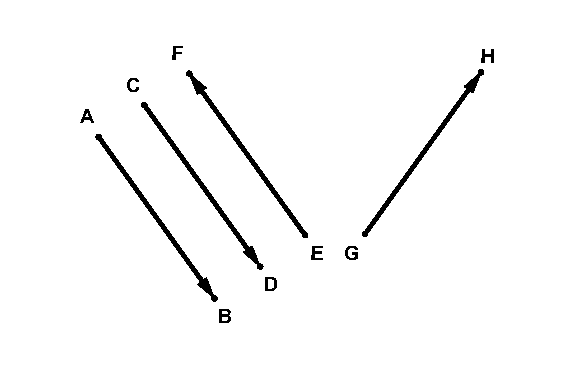
\includegraphics[scale=0.75]{./image/1.1.pdf}
    \caption{}
    \label{fig:1.1}
\end{figure}

与给定箭头相等的所有箭头的集合,称为该箭头的(几何)矢量,通常用符号$\bb{v}$表示。矢量是等价类的一个例子,按照惯例,矢量表示为等价类中任意一个箭头。

等价类,它是一个比你想象的还要更为你所熟知(并且有用)的概念。现在假设我们希望在计算机上对有理数做精确的算术运算。那么比如说,$\frac{2}{3}$就必须以$(2,3)$这样的有序对形式被计算机所读取。我们通过判断是否$ad=bc$,来测试存储在计算机中的两对有序整数$(a,b)$和$(c,d)$的等价性。这样做时,我们默认使用有理数$a/b$的定义作为所有有序整数对$(c,d)$的等价类,使得ad = be。

在实践中,将一个“数字”(如三分之二)与它的各种表示方法(如2/3、4/6等)混用是很方便的(而且很少会引起问题)。同样,当我们使用术语“矢量”时,我们指的是一个“箭头”(反之亦然),这需要读者依靠上下文来做出正确的解释。因此,在图\eqref{fig:1.2}中,我们称任何一个等价的箭头为矢量$\bb{v}$。

\begin{figure}[htbp]
	\centering
	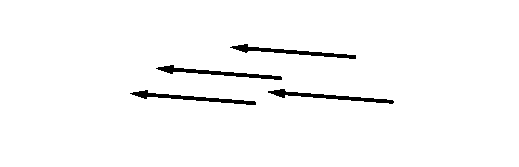
\includegraphics[scale=1.3]{./image/1.2.pdf}
	\caption{}
	\label{fig:1.2}
\end{figure}

矢量的长度$\bb{v}$由$\left| \bb{v} \right|$表示,并定义其为任意一个箭头的长度。零矢量$\bb{0}$是具有零长度的唯一矢量。我们称单位矢量
\begin{equation}
    \widehat{\bb{v}}=\frac{\bb{v}}{\left| \bb{v} \right|},\bb{v}\ne 0
\end{equation}
为矢量$\bb{v}$的方向矢量;零矢量$\bb{0}$没有方向。

我们可以任意在$E_3$中选择一点$O$,并将其称为原点。从点$O$到点$P$(的箭头)的矢量$\bb{x}$称为$P$的位置。我们有时将“位置是$\bb{x}$的点$P$”简写成$P(\bb{x})$。

\section{两矢量之和}

两个矢量$\bb{u}$和$\bb{v}$的加法可以用两种等价的方式定义\footnote{这两个定义的等价性和唯一性可以从欧氏几何的公设中得到证明:。}。

方式1:三角形法则(图\eqref{fig:1.3}a)。 取代表$\bb{u}$的任何一个箭头,比如$\rr{AB}$。选定后,将有且仅有一个箭头$\rr{BC}$代表$\bb{v}$;$\bb{u}+\bb{v}$被定义为箭头$\rr{AC}$的矢量。如果在使用中希望添加一串矢量(练习1.1),那么这个定义就比较方便,但它无法清晰的体现出矢量加法的交换性。出于对称的原因,最好使用以下定义。

\begin{figure}[htbp]
	\centering
	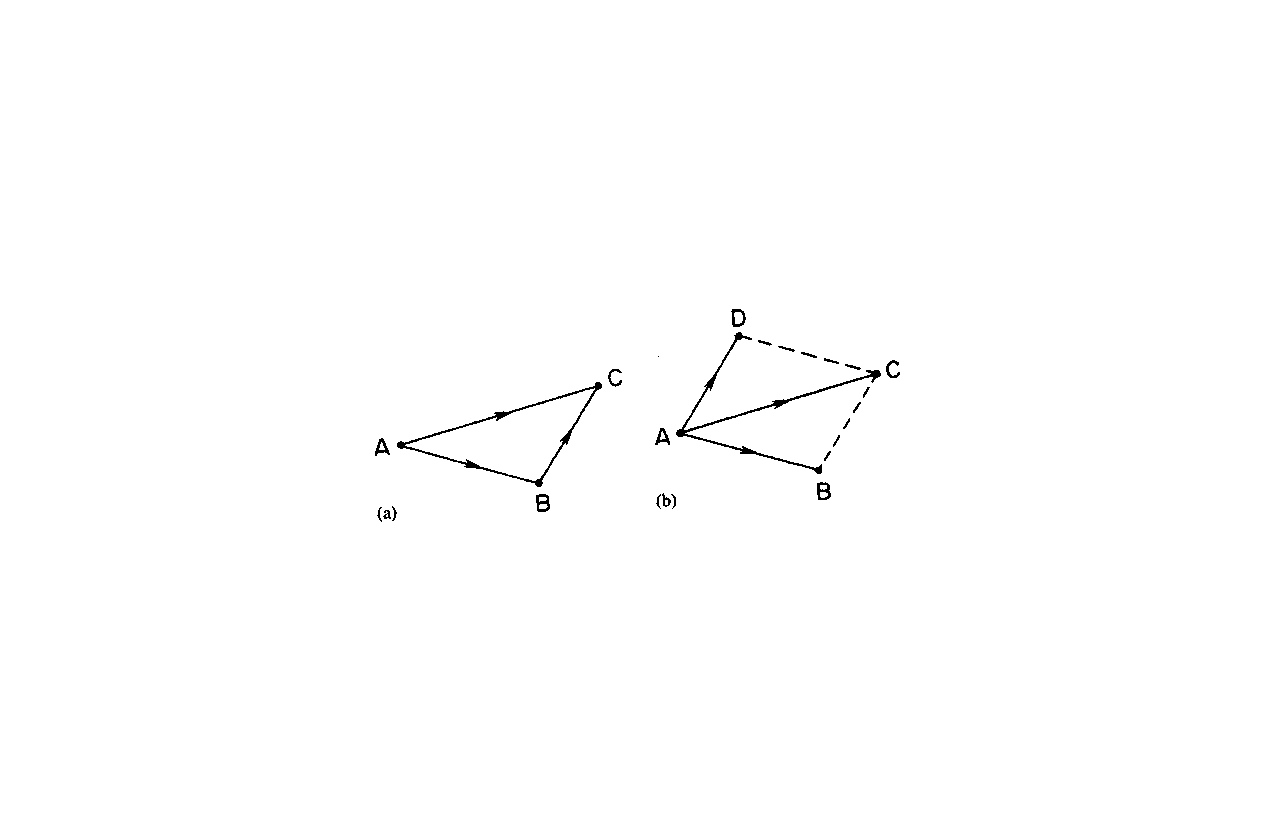
\includegraphics{./image/1.3.pdf}
	\caption{}
	\label{fig:1.3}
\end{figure}

方式2:平行四边形法则(图\eqref{fig:1.3}b)。设$\bb{u}$和$\bb{v}$由任意两个尾端重合的箭头表示,比如$\rr{AB}$和$\rr{AD}$。那么$\bb{u}+\bb{v}$是箭头$\rr{AC}$的矢量,其中$C$是平行四边形的$A$对面的顶点,$\rr{AB}$和$\rr{AD}$为共尾端箭头。

以这种方式添加三个或更多矢量在图形上有点笨拙,但$\bb{u}+\bb{v}+\bb{w}$在三维空间中有以下简洁的解释。令$\bb{u}$、$\bb{v}$和$\bb{w}$由箭头$\rr{AB}$、$\rr{AC}$和$\rr{AD}$表示。 那么对于这个尾端位于$A$,躺在以$\rr{AB}$、$\rr{AC}$和$\rr{AD}$为共端边的平行六面体的对角线上的箭头,$\bb{u}+\bb{v}+\bb{w}$是它的矢量。见练习1.2。

\section{\texorpdfstring{标量$\alpha$与矢量$\bb{v}$的乘法}{标量α与矢量v的乘法}}

矢量$\bb{v}$与标量$\alpha$的乘法以一种直观的方式定义:如果$\rr{AB}$是表示$\bb{v}$的箭头,则 $\alpha \bb{v}$是箭头$\alpha \rr{AB}$的矢量,(可以回想一下,在欧几里德几何中,我们借助相似三角形进行乘法运算) .

所有几何矢量的集合,连同标量的加法和乘法运算,形成一个矢量空间。 线性矢量空间的其他常见示例有:所有$n$次多项式的集合、$n$阶线性齐次微分方程的所有解集以及所有$m\times n$矩阵的集合以及标量的加法和乘法的定义。

\section{矢量可以表示的东西}

许多物理和运动学对象——从一点到另一点的位移、作用在粒子上的力、刚体绕轴的有限旋转——都有方向和大小。 我们可以用矢量来表示这些属性\footnote{诸如“表示力的属性的矢量$\bb{F}$”之类的短语用来描述力的性质是精确的。 为了方便,我们可以将其简化为“表示力的矢量 $\bb{F}$”,甚至可以简化为“力$\bb{F}$”。 当上下文表述清晰时,简短的“$\bb{F}$”可能就足够了。},在这样做时,我们必须牢记两个基本点。

\begin{figure}[htbp]
	\centering
	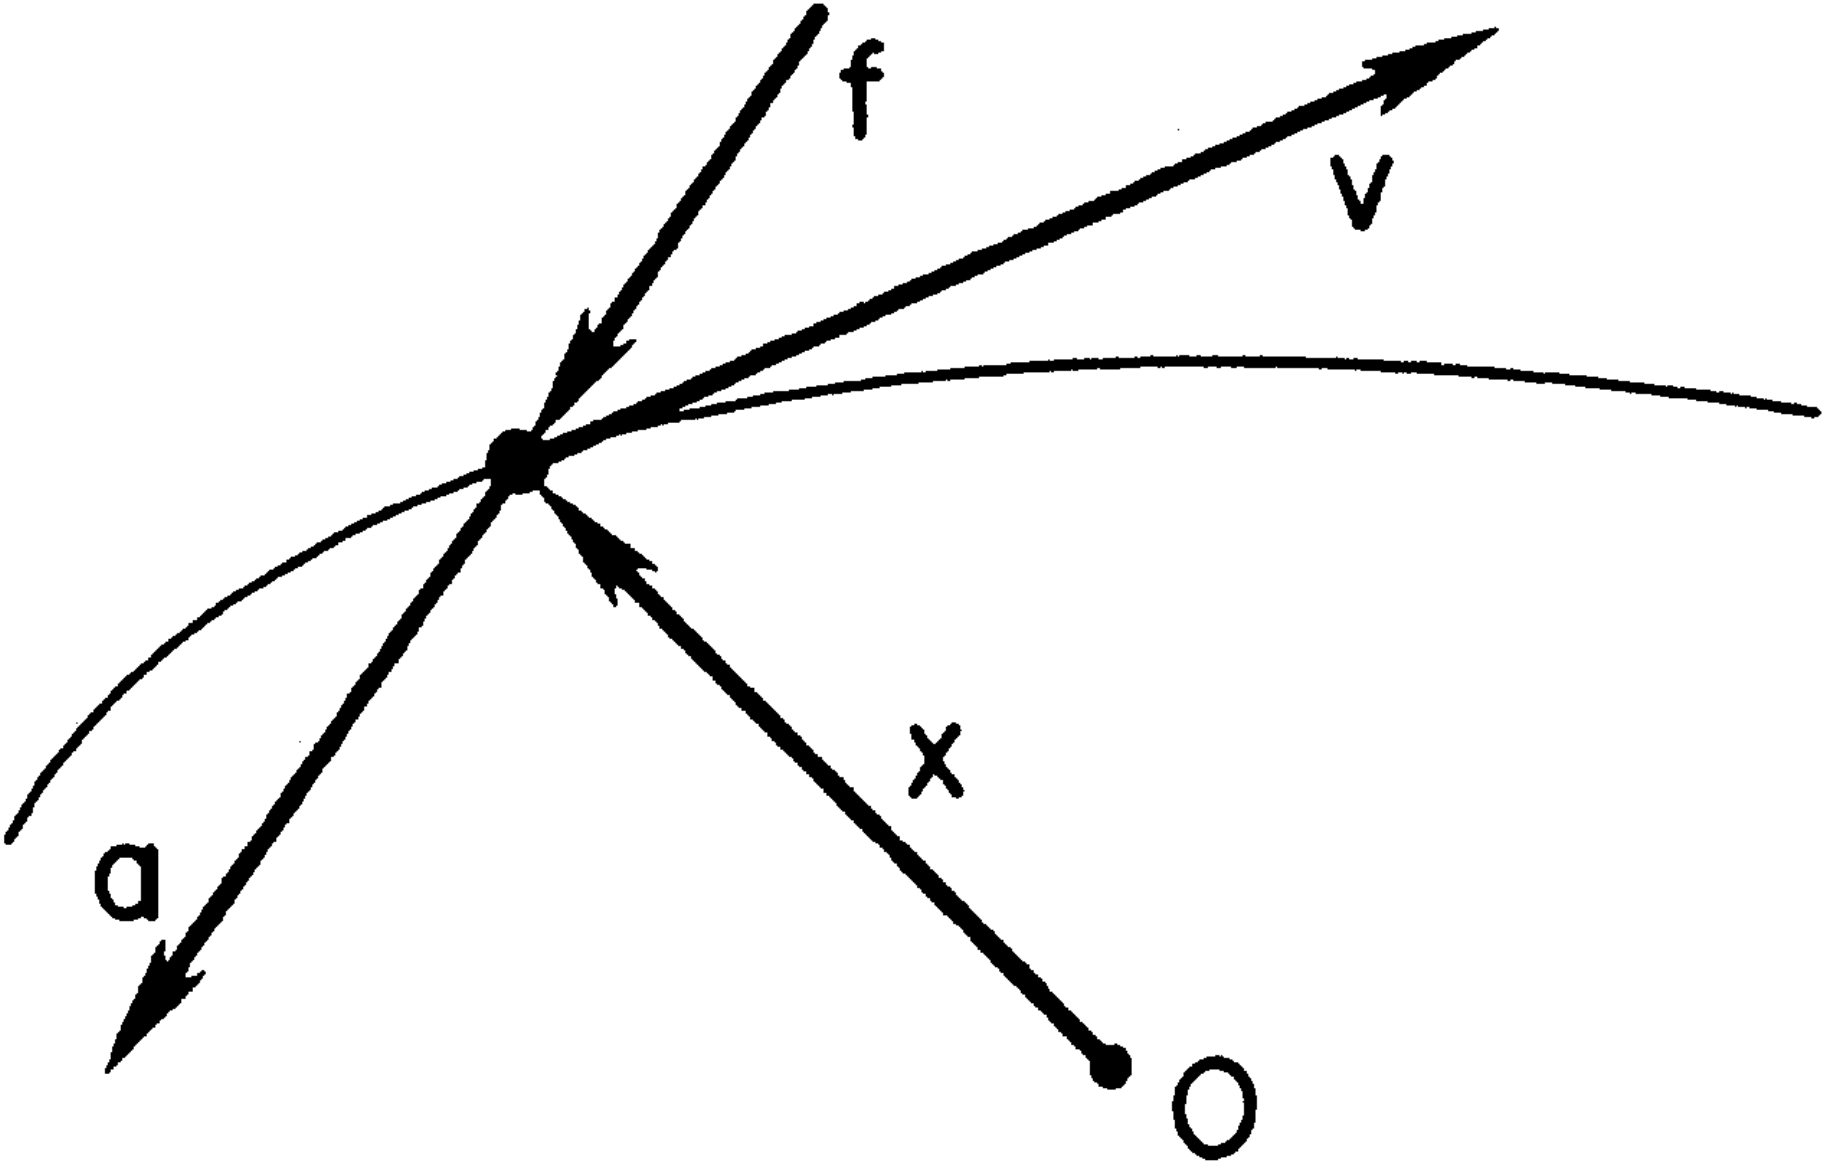
\includegraphics[width=0.4\textwidth]{./image/1.4.png}
	\caption{}
	\label{fig:1.4}
\end{figure}

重点1:\textbf{不同类型的对象由属于不同矢量空间的矢量表示。}否则,我们可以将力与位移混为一谈。不过,为了简洁明了,我们经常将不同类型的矢量放在同一张图片中,如图\eqref{fig:1.4}所示,它显示了在空中飞行的炮弹的位置$\bb{x}$、速度$\bb{v}$、加速度$\bb{a}$和作用其上的力$\bb{F}$。


重点2:\textbf{矢量加法不一定能反映物体的属性。}对于位移、力或速度,矢量加法有明显的物理含义;对于刚体围绕固定点的连续有限旋转,则没有。关于矢量加法,我们将在后文详述\footnote{物理学中,位移、力和速度的相加方式存在差异:位移遵循三角线法则,力在公共点处遵循平行四边形法则,而速度“像矢量相加”只是因为连续介质力学考虑了运动参考系这一假设。在相对论中,速度不相加。}。

\section{笛卡尔坐标系}

多亏了笛卡尔,我们可以如下文所示,用代数语言来描述三维欧几里德空间的特征。通过原点$O$绘制任意三条相互垂直($\bot $)的线。将其中一条线称为$x$轴,并在其上放置一个点$I\ne 0$。从$O$开始包含$I$的射线(或称半线)称为正$x$轴。$\rr{OI}$称为沿$x$轴的单位箭头,我们用$\bf{e}_x$来表示。在余下的线中选择一条,将其称为$y$轴,并在其上放置一个点$J$,使得$\rr{OJ}$的长度等于$\rr{OI}$。$\rr{OJ}$称为$y$轴的单位箭头,我们用$\bf{e}_y$表示它的矢量。通过$O$的最后一条线称为$z$轴,通过任意采用右手法则,我们可以放置一个唯一点$K$在$z$轴上\footnote{这意味着如果我们将右手的手指从$\rr{OI}$向$\rr{OJ}$弯曲,那么我们的拇指将指向$\rr{OK}$的方向。},使得$\rr{OK}$的长度等于$\rr{OI}$的长度。$\rr{OK}$是$z$单位箭头,$\bf{e}_z$表示其矢量。

任何点$P$都可以用有序三元实数组$(x,y,z)$表示,称为$P$的笛卡尔坐标。第一个数字或$x$坐标是其与$yz$平面的垂直距离。因此,如果$P$与$I$位于$yz$平面的同一侧,则$x$为正;如果位于另一侧,则$x$为负;如果$P$位于$yz$平面内,则$x$为零。第二个和第三个坐标$y$和$z$以类似的方式定义。为了表示点$P$的坐标为$(x,y,z)$,我们有时会写成$P(x,y,z)$。

当矢量$\bb{v}$由尾端为原点$O$的箭头表示时,则此箭头的首端坐标$(v_x,v_y,v_z)$称为$\bb{v}$的笛卡尔坐标,写作$\bb{v}\sim (v_x,v_y,v_z)$。因此,
\begin{align}
	\bf{e}_x\sim \left( 1,0,0 \right) ,\bf{e}_y\sim &\left( 0,1,0 \right) ,\bf{e}_z\sim \left( 0,0,1 \right)\label{equ:1.2}\\
	\bb{x}\sim &\left( x,y,z \right)\label{equ:1.3}
\end{align}
有了将笛卡尔坐标$(v_x,v_y,v_z)$分配给矢量$\bb{v}$的方法,反之,我们可以很容易地推导出以下关系:
\begin{enumerate}[(i)]
    \item 根据勾股定理\footnote{这里我们从$E_3$的几何特性中推导出了$E_3$的代数特性。换句话说,在很多方面情况下,我们将$E_3$定义为所有有序三元实数组$(x,y,z)$的集合,问题会更简单,而任意两点$(x_1,y_1,z_1)$和 $(x_2,y_2,z_2)$之间的距离由下式给出
    \begin{equation*}
        \sqrt{\left( x_1-x_2 \right) ^2+\left( y_1-y_2 \right) ^2+\left( z_1-z_2 \right) ^2}
    \end{equation*}
    }
    \begin{equation}\label{equ:1.4}
        \left| \bb{v} \right|=\sqrt{v_{x}^{2}+v_{y}^{2}+x_{z}^{2}}
    \end{equation}
    \item 若$\alpha$为实数,则
    \begin{equation}\label{equ:1.5}
        \alpha \bb{v}\sim (\alpha v_x,\alpha v_y,\alpha v_z)
    \end{equation}
    \item 若$\bb{w}\sim \left( w_x,w_y,w_z \right) $,则
    \begin{equation}\label{equ:1.6}
        \bb{w}\pm \bb{v}\sim (w_x\pm v_x,w_y\pm v_y,w_z\pm v_z)
    \end{equation}
    \item 
    \begin{equation}\label{equ:1.7}
        \bb{v}=\bb{w}\Longleftrightarrow w_x=v_x,w_y=v_y,w_z=v_z
    \end{equation}
\end{enumerate}

\section{点积}
两个矢量$\bb{u}$和$\bb{v}$的点积写作$\bb{u}\cdot \bb{v}$,它在物理学和几何学著作中广泛出现\footnote{当我们尝试从物理上解释点积时,需要考虑某些技术细节。 请参阅本章末尾的讨论。}。一些作者会用这样的公式来定义点积
\begin{equation}
    \bb{u}\cdot \bb{v}=\left| \bb{u} \right|\left| \bb{v} \right|\cos \theta \,\, ,  0\le \theta \le \pi \label{equ:1.8} 
\end{equation}
其中,$\theta$表示两个矢量$\bb{u}$和$\bb{v}$之间的夹角。这个定义看起来简洁有力。诶,等一下。我们只知道如何计算得到一个矢量的长度,夹角$\theta $该如何得到呢?事实上,我们没有办法,这里我们只能将式\eqref{equ:1.8}作为夹角$\theta $的定义。因此我们需要想出一个不依赖于$\theta$的,关于$\bb{u}\cdot \bb{v}$的定义。

\begin{figure}[htbp]
	\centering
	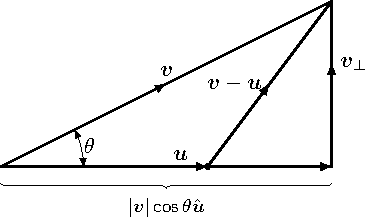
\includegraphics[width=0.4\textwidth]{./image/1.5.pdf}
	\caption{}
	\label{fig:1.5}
\end{figure}

如果$\left| \bb{u} \right|\left| \bb{v} \right| = 0$,则有$\bb{u}\cdot \bb{v}=0$。参考图\eqref{fig:1.5},一般情况下的点积定义可以用严格的几何方法来构造。图中的双向箭头反映无论两个矢量$\bb{u}$和$\bb{v}$之间的相对位置如何,夹角$\theta $恒为非负值。如图所示,矢量$\bb{v}$可以表示为矢量$\left| \bb{v} \right|\cos \theta \widehat{\bb{u}}$(它平行于$\bb{u}$)与矢量$\bb{v}_{\bot}$(它垂直于$\bb{u}$)之和。先利用两个直角三角形中较大的那一个,再利用另一个,根据勾股定理可以得到
\begin{align}
	\left| \bb{v} \right|^2&=\left| \bb{v} \right|^2\cos ^2\theta +\left| \bb{v}_{\bot} \right|^2,\label{equ:1.9}\\
	\left| \bb{v}-\bb{u} \right|^2&=\left( \left| \bb{v} \right|\cos \theta -\left| \bb{u} \right| \right) ^2+\left| \bb{v}_{\bot} \right|^2\nonumber\\
	\left| \bb{v}-\bb{u} \right|^2&=\left| \bb{v} \right|^2\cos ^2\theta -2\left| \bb{u} \right|\left| \bb{v} \right|\cos \theta +\left| \bb{u} \right|^2+\left| \bb{v}_{\bot} \right|^2\nonumber\\
	\footnotemark&=\left| \bb{u} \right|^2+\left| \bb{v} \right|^2-2\left| \bb{u} \right|\left| \bb{v} \right|\cos \theta \label{equ:1.10},
\end{align}
\footnotetext{这个结论一般被称作余弦定理。}

根据式\eqref{equ:1.9},对比式\eqref{equ:1.8}与式\eqref{equ:1.10},我们可以导出定义
\begin{equation}\label{equ:1.11}
    \bb{u}\cdot \bb{v}=\frac{1}{2}\left( \left| \bb{u} \right|^2+\left| \bb{v} \right|^2-\left| \bb{v}-\bb{u} \right|^2 \right) 
\end{equation}
注意,若$\left| \bb{u} \right|\left| \bb{v} \right| = 0$,则$\bb{u}\cdot \bb{v}=0$,这与我们用之前的定义导出的结果一致。若$\bb{u}=\bb{v}$,则
\begin{equation}
    \bb{v}\cdot \bb{v}=\left| \bb{v} \right|^2
\end{equation}
若两个矢量的点积等于0,那么这两个矢量彼此垂直。

为了用计算机计算两个矢量的点积,我们需要写出点积的分量表达式。这很简单。若$\bb{u}\sim \left( u_x,u_y,u_z \right)$ ,$\bb{v}\sim \left( v_x,v_y,v_z \right) $,则根据式\eqref{equ:1.4}以及式\eqref{equ:1.11}
\begin{equation}\label{equ:1.13}
    \bb{u}\cdot \bb{v}=u_xv_x+u_yv_y+u_zv_z
\end{equation}

假设在不改变$\bb{u}$和$\bb{v}$的情况下,我们引入另一组笛卡尔坐标系。 通常,$\bb{u}$和$\bb{v}$相对于新轴的分量会有所不同,但式\eqref{equ:1.13}的右侧会发生变化吗?作为分量乘积的每一个单项当然会变,但它们的总和不会。为什么? 因为\eqref{equ:1.11}是根据长度定义$\bb{u}\cdot \bb{v}$的,而在欧几里德几何中,长度定义不受所选坐标系的影响。因此,我们说点积是一个几何不变量。

点积的另一个关键属性是它满足分配率,也就是说
\begin{equation}\label{equ:1.14}
	\bb{u}\cdot \left( \bb{v}+\bb{w} \right) =\bb{u}\cdot \bb{v}+\bb{u}\cdot \bb{w}\,\, ,  \forall \bb{u},\bb{v},\bb{w}
\end{equation}
为了证明:式\eqref{equ:1.14},我们设$\bb{w}\sim \left( w_x,w_y,w_z \right) $。根据式\eqref{equ:1.13},则有
\begin{align*}
	\bb{u}\cdot \left( \bb{v}+\bb{w} \right) &=u_x\left( v_x+w_x \right) +u_y\left( v_y+w_y \right) +u_z\left( v_z+w_z \right)\\
	&=u_xv_x+u_yv_y+u_zv_z+u_xw_x+u_yw_y+u_zw_z\\
	&=\bb{u}\cdot \bb{v}+\bb{u}\cdot \bb{w}
\end{align*}
\qed

这个证明:的过程说明了一个很重要的问题:一般情况下,一个几何定理最适合在笛卡尔坐标系中来证明:。相应的,由于式\eqref{equ:1.14}的结论与具体的坐标系无关,因此它直接推自式\eqref{equ:1.11}。可以参考练习1.7。记住,对于一个问题,既要从几何方面思考,也要从代数方面思考,虽然可能某一种方法的证明:相较于另一种更加困难,但是也可能会带来新的思考与新的收获。

\begin{example}
若$\bb{u}\sim \left( 1,2,3 \right) $,$\bb{v}\sim \left( -3,1,-2 \right) $,计算$\bb{u}\cdot \bb{v}$的值和它们的夹角。
\end{example}
\begin{solution}
根据式\eqref{equ:1.14}
\begin{equation*}
	\bb{u}\cdot \bb{v}=\left( 1 \right) \left( -3 \right) +\left( 2 \right) \left( 1 \right) +\left( 3 \right) \left( -2 \right) =-7
\end{equation*}
并由式\eqref{equ:1.8}
\begin{equation*}
	\theta =\arccos \frac{\bb{u}\cdot \bb{v}}{\left| \bb{u} \right|\left| \bb{v} \right|}\,\, ,  0\le \theta \le \pi 
\end{equation*}
此时
\begin{align*}
	\left| \bb{u} \right|&=\sqrt{1^2+2^2+3^2}=\sqrt{14}\\
	\left| \bb{v} \right|&=\sqrt{\left( -3 \right) ^2+1^2+\left( -2 \right) ^2}=\sqrt{14}
\end{align*}
因此
\begin{equation*}
	\theta =\arccos \left( -7/14 \right) =120\degree=\frac{2}{3}\pi 
\end{equation*}
\end{solution}

\section{笛卡尔基矢量}
若已知任意一个矢量$\bb{v}$的分量$(v_x,v_y,v_z)$,根据式\eqref{equ:1.6}与式\eqref{equ:1.5},我们置
\begin{equation}\label{equ:1.15}
    \begin{aligned}
        \left( v_x,v_y,v_z \right) &=\left( v_x,0,0 \right) +\left( 0,v_y,0 \right) +\left( 0,0,v_z \right)\\
        &=v_x\left( 1,0,0 \right) +v_y\left( 0,1,0 \right) +v_z\left( 0,0,1 \right)
    \end{aligned}
\end{equation}
回想式\eqref{equ:1.2}和式\eqref{equ:1.6},我们可以推出$\bb{v}$有唯一的表达式
\begin{equation}\label{equ:1.16}
    \bb{v}=v_x\bf{e}_x+v_y\bf{e}_y+v_z\bf{e}_z
\end{equation}
矢量集${\bf{e}_x,\bf{e}_y,\bf{e}_z}$被称作\textbf{标准笛卡尔基},而它的元素即为笛卡尔基矢量。矢量$\bb{v}$的笛卡尔坐标也可以称作$\bb{v}$相对于${\bf{e}_x,\bf{e}_y,\bf{e}_z}$的分量。

\section{矢量加法的物理意义}

这里有必要强调作为物理或运动学属性的反映的矢量加法与在式\eqref{equ:1.6}右侧所使用的矢量加法之间的差别。例如,我们设$\bb{v}$表示刚体绕定点的转动。根据右手法则,取$\bb{v}$的方向与大小分别代表转轴与转动角度。如果随后又发生了一次转动,用矢量$\bb{u}$表示,那么从运动学的角度考虑,这两次连续的转动得到的效果可以用一次转动予以替代,我们设为$\bb{w}$。然而,通常来讲$\bb{v}+\bb{u}\ne \bb{w}$,换言之,连续有限转动不能如矢量一般叠加\footnote{转动也可以用矩阵来表示。如果两个连续的旋转由矩阵$V$和$U$表示,则它们等效于由矩阵$W = UV$表示的单个旋转。$u$、$v$或$w$可以记作$U$、$V$或$W$的实特征向量。}。不过,如果我们不将矢量的求和解释为旋转的叠加,那么式\eqref{equ:1.6}右侧的加法就是有意义的。我可以试着用一个简单的比喻来说明这一点。假设一个教室里有20个学生和30把椅子。从统计学角度来讲,我们可以说 "每把椅子上有$\frac{2}{3}$个学生",尽管在现实生活中并不存在$\frac{2}{3}$个学生。这是因为我们用整数来代替了学生和椅子的数量,为了得到统计数据,我们就需要按照计算法则来计算这些整数。

比方说,当矢量$\bb{v}$如式\eqref{equ:1.16}中所示表示力的时候,矢量加法就可以反映物理性质。“力具有矢量叠加性”是一个实验事实。参考练习1.3。在这种情况下,数学意义上的矢量分解恰好有一个直接的物理解释。这里再举一个例子,一个餐厅有20瓶1加仑的牛奶和30个罐子,此时,我们不止可以从数学意义上讲“每个罐子有$\frac{2}{3}$加仑的牛奶”,在实际中,我们也确实可以让每个罐子盛$\frac{2}{3}$加仑的牛奶。这里,数学意义上的整数除法就有一个对应的物理意义。

\section{叉积}

叉积的应用十分广泛:例如力学中我们想计算力矩,我们会用到叉积;电磁学中我们想计算运动电荷在磁场中所受的力,我们会用到叉积;几何学中我们想计算平行六面体或四面体的体积,我们会用到叉积,以及在物理学和几何学中的其他许多领域,我们会还用到叉积\footnote{前面关于点积的物理解释的注记也适用于叉积。请参见本章末尾的讨论。}。

两个矢量$\bb{u}$和$\bb{v}$的叉积记作$\bb{u}\times \bb{v}$,定义为一个指向以$\bb{u}$和$\bb{v}$为共端边平行四边形右侧区域的矢量。其满足
\begin{equation}
    \left| \bb{u}\times \bb{v} \right|=\left| \bb{u} \right|\left| \bb{v} \right|\sin \theta \,\, ,  0\le \theta \le \pi 
\end{equation}
其中$\bb{u}\times \bb{v}$的方向为,当右手四指从$\bb{u}$弯向$\bb{v}$时,大拇指所指的方向。图\eqref{fig:1.6}指出了两种可能的情况。

根据叉积的定义,我们有
\begin{equation}
    \bb{u}\times \bb{v}=-\bb{v}\times \bb{u}
\end{equation}

\begin{figure}[htbp]
    \centering
    \begin{minipage}[b]{0.48\textwidth}
        \centering
        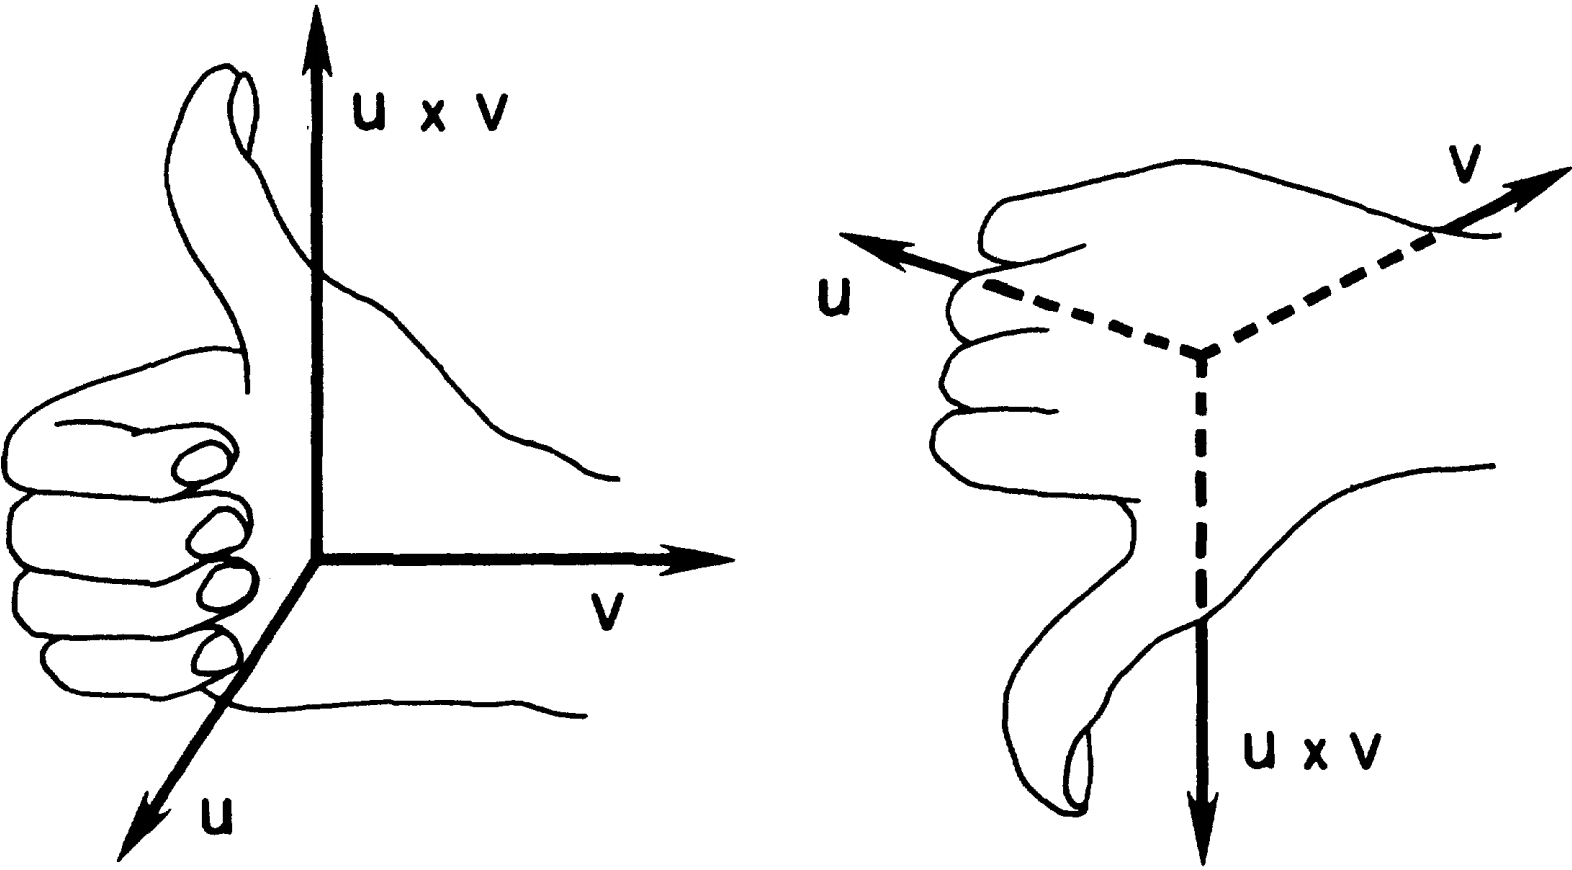
\includegraphics[width=0.85\textwidth]{./image/1.6.png}
        \caption{}
        \label{fig:1.6}
    \end{minipage}
    \begin{minipage}[b]{0.48\textwidth}
        \centering
        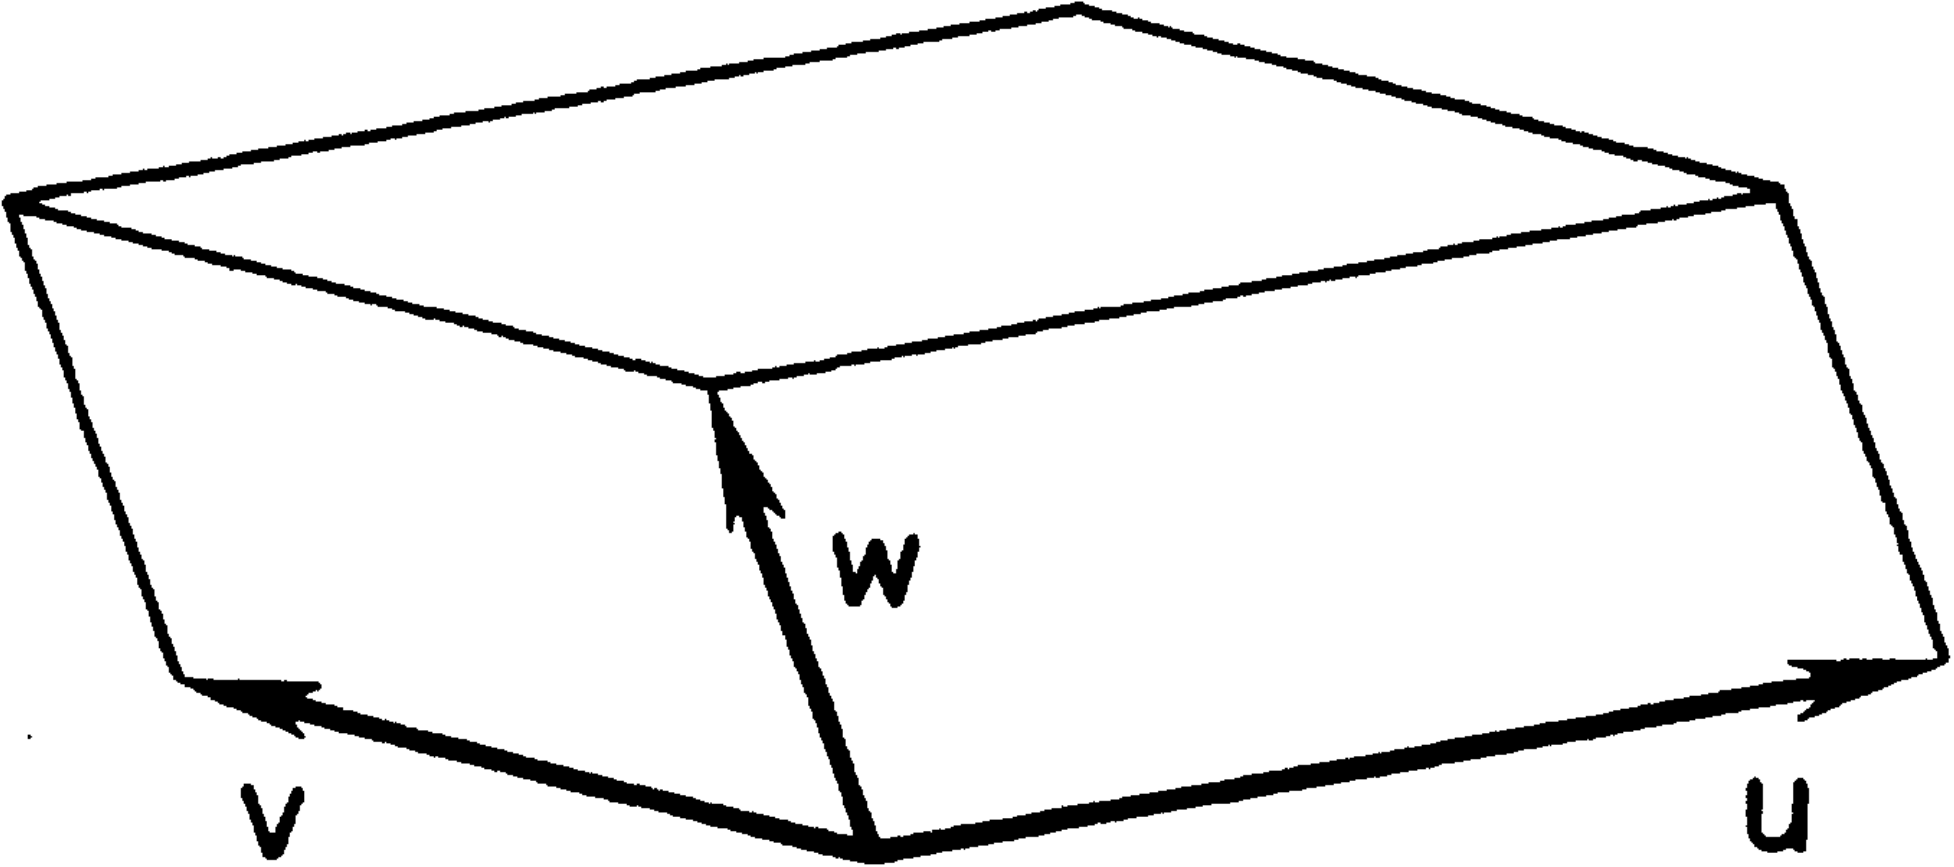
\includegraphics[width=0.85\textwidth]{./image/1.7.png}
        \caption{}
        \label{fig:1.7}
    \end{minipage}
\end{figure}

叉积进一步的用途在于三重混合积$(\bb{u}\times \bb{v})\cdot \bb{w}$的几何含义。考虑一个以$\bb{u}$、$\bb{v}$和$\bb{w}$作为共端边缘的平行六面体,将它的体积记作$\mathrm{vol}\left( \bb{u},\bb{v},\bb{w} \right) $。我们将平行六面体分割成一片片的片元,每一个片元的高度极小而底面都是$\bb{u}$和$\bb{v}$构成的平行四边形\footnote{几乎不需要微积分我们就给出这个模型。想象一副相同的牌,每一张都是平行四边形。纸牌组的体积是它的厚度乘以纸牌面的面积,如果纸牌组被剪切成平行六面体的形状,这个体积显然是没有变化的。(译者注:即祖逖原理。)},通过这样分割,我们有
\begin{equation}
    \mathrm{vol}\left( \bb{u},\bb{v},\bb{w} \right) =\left| \left( \bb{u}\times \bb{v} \right) \cdot \bb{w} \right|
\end{equation}
如果$(\bb{u},\bb{v},\bb{w})$以这样的顺序组成了一个右手系,如图\eqref{fig:1.7}所示,那么根据几何学我们可以得到
\begin{equation}\label{equ:1.20}
    \mathrm{vol}\left( \bb{u},\bb{v},\bb{w} \right) =\left( \bb{u}\times \bb{v} \right) \cdot \bb{w}=\left( \bb{v}\times \bb{w} \right) \cdot \bb{u}=\left( \bb{w}\times \bb{u} \right) \cdot \bb{v} \le 0
\end{equation}
换言之,$\left( \bb{u}\times \bb{v} \right) \cdot \bb{w}$具有轮换对称性。

借助式\eqref{equ:1.20}我们将证明:叉积服从加法分配律
\begin{equation}\label{equ:1.21}
    \bb{u}\times \left( \bb{v}+\bb{w} \right) =\bb{u}\times \bb{v}+\bb{u}\times \bb{w}
\end{equation}
为此,我们引入一个定理:两个矢量相等,当且仅当它们与任意一个矢量$\bb{c}$的点积相等\footnote{为什么?好吧,我们来证明:。首先,如果已知$\bb{u}=\bb{v}$,那么由此可推出,对于任意矢量$\bb{c}$,$\bb{u}\cdot \bb{c}=\bb{v}\cdot \bb{c}$都成立;反过来讲,若已知对于任意矢量$\bb{c}$,$\bb{u}\cdot \bb{c}=\bb{v}\cdot \bb{c}$都成立,我们可以设$\bb{c}=\bb{u}-\bb{v}$,此时有
\begin{align*}
	\bb{u}\cdot \bb{c}&=\bb{v}\cdot \bb{c}\\
	\bb{u}\cdot \bb{c}-\bb{v}\cdot \bb{c}&=0\\
	\left( \bb{u}-\bb{v} \right) \cdot \left( \bb{u}-\bb{v} \right) &=0\\
	\left| \bb{u}-\bb{v} \right|^2&=0
\end{align*}
可以导出$\bb{u}-\bb{v}=0$,也就是说,$\bb{u}=\bb{v}$。
}。由此

\begin{align*}
	\left[ \bb{u}\times \left( \bb{v}+\bb{w} \right) \right] \cdot \bb{c}&=\left( \bb{c}\times \bb{u} \right) \cdot \left( \bb{v}+\bb{w} \right)\\
	&=\left( \bb{c}\times \bb{u} \right) \cdot \bb{v}+\left( \bb{c}\times \bb{u} \right) \cdot \bb{w}\\
	&=\left( \bb{u}\times \bb{v} \right) \cdot \bb{c}+\left( \bb{u}\times \bb{w} \right) \cdot \bb{c}\\
	&=\left( \bb{u}\times \bb{v}+\bb{u}\times \bb{w} \right) \cdot \bb{c}
\end{align*}
\qed

\begin{example}
    不用分量,证明:三重矢积公式:
    \begin{equation}\label{equ:1.22}
        \left( \bb{u}\times \bb{v} \right) \times \bb{w}=\left( \bb{w}\cdot \bb{u} \right) \bb{v}-\left( \bb{w}\cdot \bb{v} \right) \bb{u}
    \end{equation}
\end{example}
\begin{solution}
    $\bb{u}\times \bb{v}$必然垂直于$\bb{u}$、$\bb{v}$所在平面。因此,$\left( \bb{u}\times \bb{v} \right) \times \bb{w}$必然垂直于$\left( \bb{u}\times \bb{v} \right) $、$\bb{w}$所在平面,躺在$\bb{u}$、$\bb{v}$所在平面上,因此我们设
    \begin{equation}\label{equ:Example 1.2*}
         \left( \bb{u}\times \bb{v} \right) \times \bb{w}=A\bb{u}+B\bb{v}\tag{*}
    \end{equation}
    其中,$A$、$B$为关于$\bb{u},\bb{v},\bb{w}$的未知标量函数。式\eqref{equ:Example 1.2*}的左边垂直于$\bb{w}$,因此可以得到
    \begin{equation*}
        0=A\bb{u}\cdot \bb{w}+B\bb{v}\cdot \bb{w}
    \end{equation*}
    我们设
    \begin{equation*}
        A=-C\left( \bb{v}\cdot \bb{w} \right) \,\, ,  B=C\left( \bb{u}\cdot \bb{w} \right) 
    \end{equation*}
    其中,$C$为关于$\bb{u},\bb{v},\bb{w}$的未知标量函数。因此
    \begin{equation}\label{equ:Example 1.2**}
         \left( \bb{u}\times \bb{v} \right) \times \bb{w}=C\left( \bb{u},\bb{v},\bb{w} \right) \left[ \left( \bb{u}\cdot \bb{w} \right) \bb{v}-\left( \bb{v}\cdot \bb{w} \right) \bb{u} \right] \tag{**}
    \end{equation}
    特别地,当$\bb{w}=\bb{u}$时,式\eqref{equ:Example 1.2**}简化为
    \begin{equation}\label{equ:Example 1.2***}
         \left( \bb{u}\times \bb{v} \right) \times \bb{u}=C\left( \bb{u},\bb{v},\bb{u} \right) \left[ \left| \bb{u} \right|^2\bb{v}-\left( \bb{v}\cdot \bb{u} \right) \bb{u} \right] \tag{$\begin{subarray}{c}
            *\\
            **
        \end{subarray}$}
    \end{equation}
    用$\bb{v}$点乘等式两边,并对左边进行整理,我们可以得到
    \begin{equation}\label{equ:Example 1.2****}
         \left( \bb{u}\times \bb{v} \right) \cdot \left( \bb{u}\times \bb{v} \right) =C\left( \bb{u},\bb{v},\bb{u} \right) \left[ \left| \bb{u} \right|^2\left| \bb{v} \right|^2-\left( \bb{u}\cdot \bb{v} \right) ^2 \right] \tag{$\begin{subarray}{c}
            **\\
            **
        \end{subarray}$}
    \end{equation}
    但是
    \begin{align*}
        \left( \bb{u}\times \bb{v} \right) \cdot \left( \bb{u}\times \bb{v} \right) &=\left| \bb{u}\times \bb{v} \right|^2\\
        &=\left| \bb{u} \right|^2\left| \bb{v} \right|^2\sin ^2\theta\\
        &=\left| \bb{u} \right|^2\left| \bb{v} \right|^2\left( 1-\cos ^2\theta \right)\\
        &=\left| \bb{u} \right|^2\left| \bb{v} \right|^2-\left( \bb{u}\cdot \bb{v} \right) ^2
    \end{align*}
    对比这个表达式的最后一行和式\eqref{equ:Example 1.2****}的右边,我们可以得到${ C\left( \bb{u},\bb{v},\bb{u} \right) =1}$。

    现在,用$\bb{u}$点乘式\eqref{equ:Example 1.2**}两边,整理左边的三重标积,我们有
    \begin{equation*}
        \left[ \bb{u}\times \left( \bb{u}\times \bb{v} \right) \right] \cdot \bb{w}=C\left( \bb{u},\bb{v},\bb{w} \right) \left[ \left( \bb{u}\cdot \bb{w} \right) \left( \bb{v}\cdot \bb{u} \right) -\left( \bb{v}\cdot \bb{w} \right) \left| \bb{u} \right|^2 \right] 
    \end{equation*}
    但是我们在上述讨论中得出了式\eqref{equ:Example 1.2***}中${ C\left( \bb{u},\bb{v},\bb{u} \right) =1}$,因此有
    \begin{equation*}
        \left[ \left( \bb{u}\times \bb{v} \right) \times \bb{w} \right] \cdot \bb{u}=\left( \bb{u}\cdot \bb{w} \right) \left( \bb{v}\cdot \bb{u} \right) -\left( \bb{v}\cdot \bb{w} \right) \left| \bb{u} \right|^2
    \end{equation*}

    因此${ C\left( \bb{u},\bb{v},\bb{w} \right) =1}$

    \qed
\end{solution}
在投影面积方面,三重标积有另一种实用的解释。见习题1.15。

我们如何找到$\bb{u}\times \bb{v}$的笛卡尔坐标?这不像 $\bb{u}\cdot \bb{v}$那么简单。一方面是因为,$\bb{u}\times \bb{v}$是矢量而不是标量,而另一方面,$\bb{u}\times \bb{v}$是一只生活在三维空间中的野兽!(Grassmann 创建了一个代数体系,它为高维欧几里德空间中诸如$\bb{u}\times \bb{v}$或$\bb{u}\times \bb{v}\times \bb{w}$之类的对象赋予了意义,在这些空间中,它们被称为楔积。)一种直接(但乏味)的方法是重复应用分配律\eqref{equ:1.21},我们置
\begin{align}
	\bb{u}\times \bb{v}&=\left( u_x\bf{e}_x+u_y\bf{e}_y+u_z\bf{e}_z \right) \times \left( v_x\bf{e}_x+v_y\bf{e}_y+v_z\bf{e}_z \right)\nonumber\\
	&=u_xv_x\bf{e}_x\times \bf{e}_x+u_xv_y\bf{e}_x\times \bf{e}_y+u_xv_z\bf{e}_x\times \bf{e}_z\nonumber\\
	&+u_yv_x\bf{e}_y\times \bf{e}_x+u_yv_y\bf{e}_y\times \bf{e}_y+u_yv_z\bf{e}_y\times \bf{e}_z\nonumber\\
	&+u_zv_x\bf{e}_z\times \bf{e}_x+u_zv_y\bf{e}_z\times \bf{e}_y+u_zv_z\bf{e}_z\times \bf{e}_z\label{equ:1.23}
\end{align}
(烦死啦!)但是,$\bf{e}_x\times \bf{e}_x=0,\bf{e}_x\times \bf{e}_y=\bf{e}_z,\bf{e}_x\times \bf{e}_z=-\bf{e}_y$……(画个图去!)因此式\eqref{equ:1.23}简化成
\begin{equation}\label{equ:1.24}
    \bb{u}\times \bb{v}=\bf{e}_x\left( u_yv_z-u_zv_y \right) +\bf{e}_y\left( u_zv_x-u_xv_z \right) +\bf{e}_z\left( u_xv_y-u_yv_x \right) 
\end{equation}
式\eqref{equ:1.24}一种简单的记忆方法是将它写成
\begin{equation}\label{equ:1.25}
    \bb{u}\times \bb{v}=\left| \begin{matrix}
        \bf{e}_x&		\bf{e}_y&		\bf{e}_z\\
        u_x&		u_y&		u_z\\
        v_x&		v_y&		v_z\\
    \end{matrix} \right|
\end{equation}
其中,行列式应围绕第一行展开。

从式\eqref{equ:1.24}、式\eqref{equ:1.25}和行列式的性质,即行列转置值不变,交换两行(或列)改变符号,我们得到有用的公式
\begin{equation}\label{equ:1.26}
    (\bb{u}\times \bb{v})\cdot \bb{w}=\left| \begin{matrix}
        w_x&		w_y&		w_z\\
        u_x&		u_y&		u_z\\
        v_x&		v_y&		v_z\\
    \end{matrix} \right|=\left| \begin{matrix}
        u_x&		u_y&		u_z\\
        v_x&		v_y&		v_z\\
        w_x&		w_y&		w_z\\
    \end{matrix} \right|=\left| \begin{matrix}
        u_x&		v_x&		w_x\\
        u_y&		v_y&		w_y\\
        u_z&		v_z&		w_z\\
    \end{matrix} \right|
\end{equation}

\begin{example}
    用两种方法(用叉积和不用叉积)给出一个单位矢量$\bf{e}$同时垂直于$\bb{a}\sim \left( 1,-2,3 \right) $和$\bb{b}\sim \left( -1,0,1 \right) $。
\end{example}
\begin{solution}
    如果用叉积的方法,我们寻找的矢量是
    \begin{equation*}
        \bf{e}=\pm \frac{\bb{a}\times \bb{b}}{\left| \bb{a}\times \bb{b} \right|}
    \end{equation*}
    根据式\eqref{equ:1.25}
    \begin{equation*}
        \bb{a}\times \bb{b}=\left| \begin{matrix}
            \bf{e}_x&		\bf{e}_y&		\bf{e}_z\\
            1&		-2&		3\\
            -1&		0&		1\\
        \end{matrix} \right|\sim \left( -2,-4,-2 \right) 
    \end{equation*}
    因为$\left| \bb{a}\times \bb{b} \right|=2\sqrt{6}$,因此$\bf{e}\sim \pm \left( 1/\sqrt{6},2/\sqrt{6},1/\sqrt{6} \right) $

    不用叉积的方法计算$\bf{e}$,我们可以设$\bf{e}\sim \left( a,b,c \right) $。那么我们可以得到
    \begin{equation*}
        \left\{ \begin{aligned}
            \bf{e}\cdot \bb{a}&=a-2b+3c=0\\
            \bf{e}\cdot \bb{b}&=-a+c=0\\
        \end{aligned} \right. 
    \end{equation*}
    为了使$\left| \bf{e} \right|=1$,我们可以取$a=\pm 1/\sqrt{6}$,代入即可。
\end{solution}



\section{点积与叉积的另一种解释——张量}
在物理学中,我们知道恒定力$\bb{F}$作用于位移$\bb{D}$做 $\bb{F}\cdot \bb{D}$个单位的功。与位移不同,力无法直接测量,只能测量其效果(弹簧的伸长、应变仪电阻的变化等),而且,力与位移具有不同的物理单位。这表明力——更准确地说,表示力的矢量与位移位于不同的向量空间中。如果力以磅为单位,位移以英尺为单位,那么我们在两个向量空间中任意设置单位$x$轴向箭头$\rr{OI}$分别表示一磅力和一英尺距离。现在想一想:你将如何以图形方式计算$\bb{F}\cdot \bb{D}$? 你可以首先使这两个向量空间的正$x$、$y$和$z$轴重合,然后,由于$\rr{OI}$是任意选择的,因此我们可以拉伸或收缩一个$\rr{OI}$直到与另一个重合。最后,$\bb{F}$在$\bb{D}$方向上的正交投影长度将以图形方式乘以$\left| \bb{D} \right|$,从而获得一个以英尺·磅为单位的量。

所有这些想象中的推搡是为了赋予$\bb{F}\cdot \bb{D}$一个几何意义,以便人们可以进行图形计算(这是一种古老的艺术,现在很少有人实践。)难道没有一种更简单的方式来看待事物,不仅不影响数字计算,还能更好地反映不同类型的物理对象?当然有:一个力$\bb{F}$可以被认为是一个线性函数的代表,它把任何矢量$\bb{D}$(位移)转换成一个实数(称为$\bb{F}$作用于$\bb{D}$的功)。

类似但更详细的考虑也适用于叉积。例如,假设力$\bb{F}$作用于位置为$\bb{x}$的点$P$,将围绕O点的扭矩表示为$\bb{x}\times \bb{F}$,这引出了将矢量变换成矢量的线性算子的概念。这样的算子被称为二阶张量。张量这个名字来自弹性理论,在弹性理论中,在一个负载的弹性体中,应力张量作用于与一点处体元的某个面垂直的单位矢量,并给出作用在该点的平面上的张力(即每单位面积的力)。参见练习1.20。其他重要的二阶张量包括刚体动力学中的惯性张量、弹性中的应变张量和流体动力学中的动量-通量张量。

\begin{figure}[htbp]
	\centering
	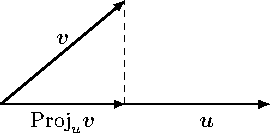
\includegraphics[width=0.4\textwidth]{./image/1.8.pdf}
	\caption{}
	\label{fig:1.8}
\end{figure}

我能想到的二阶张量的最简单且不平凡的例子如下。设向量$\bb{v}$在向量$\bb{u}$上的投影表示定义为
\begin{equation}\label{equ:1.27}
    \mathrm{Proj}_u\bb{v}=\left( \bb{v}\cdot \widehat{\bb{u}} \right) \widehat{\bb{u}}
\end{equation}

$\mathrm{Proj}_u\bb{v}$的几何含义如图\eqref{fig:1.8}所示。式\eqref{equ:1.27}的左边可以解释为算子$\mathrm{Proj}_u$作用于$\bb{v}$。式\eqref{equ:1.27} 的右边告诉我们算子$\mathrm{Proj}_u$将$\bb{v}$转换成一个$\bb{u}$方向上,大小为$\left| \bb{v}\cdot \widehat{\bb{u}} \right|$的矢量。为了符合标题中张量的要求,$\mathrm{Proj}_u$必须是线性的。但如果$\beta $和$\gamma $是任意标量,w是任意矢量,那么,根据点积的特性
\begin{align}
	\mathrm{Proj}_{\bb{u}}(\beta \bb{v}+\gamma \bb{w})&\equiv [(\beta \bb{v}+\gamma \bb{w})\cdot \widehat{\bb{u}}]\widehat{\bb{u}}\nonumber\\
	&=(\beta \bb{v}\cdot \widehat{\bb{u}}+\gamma \bb{w}\cdot \widehat{\bb{u}})\widehat{\bb{u}}\nonumber\\
	&=\beta (\bb{v}\cdot \widehat{\bb{u}})\widehat{\bb{u}}+\gamma (\bb{w}\cdot \widehat{\bb{u}})\widehat{\bb{u}}\nonumber\\
	&=\beta \mathrm{Proj}_{\bb{u}}\bb{v}+\gamma \mathrm{Proj}_{\bb{u}}\bb{w}\label{equ:1.28}
\end{align}
即$\mathrm{Proj}_u$是线性的,因此它是张量。现在做练习1.5以确保你可以在具体情况下应用这个张量。

式\eqref{equ:1.27}右边的形式反映了以下观点:两个向量$\bb{u}$和$\bb{v}$的直积$\bb{uv}$\footnote{许多作者也将直积$\bb{uv}$写作$\bb{u}\otimes \bb{v}$}是一个张量,它根据规则将任意一个向量$\bb{w}$转换成一个新的向量。
\begin{equation}\label{equ:1.29}
    \bb{uv}\left( \bb{w} \right) =\bb{u}\left( \bb{v}\cdot \bb{w} \right) 
\end{equation}
因此,特别地
\begin{equation}\label{equ:1.30}
    \mathrm{Proj}_{\bf{u}}=\widehat{\bb{u}}\widehat{\bb{u}}
\end{equation}

可以表示为直积的张量,如$\mathrm{Proj}_u$,被称为并矢。 正如我们马上要看到的,任何二阶张量都可以表示为并矢的线性组合。





\section{定义}
我们说我们得到了一个二阶张量$\bb{T}$,意味着我们知道了张量$\bb{T}$对任意一个矢量$\bb{v}$的作用(即它转换后的结果)。因此,如果有两个二阶张量$\bb{S}$和$\bb{T}$对于任意一个矢量$\bb{v}$的作用是相同的,那么$\bb{S}$和$\bb{T}$就是相等的\footnote{$\bb{T}$对$\bb{v}$的作用记为$\bb{Tv}$,$\bb{T(v)}$或是简写成$\bb{T\cdot v}$对于严谨的数学家来说,如果不提及$\bb{T}$的定义域、$\bb{T}$作用的矢量集及其范围,即$\bb{T}$将这些矢量转换后形成的向量空间,$\bb{T}$的描述是不完整的。我们假设二阶张量的定义域和范围从上下文中是显而易见的,尽管它们一般是不同的;例如,转动惯量张量的定义域是角速度空间,但它的值域是转动动量空间(见习题 4.22)。}。更正式地说,
\begin{equation}\label{equ:1.31}
    \bb{S}=\bb{T}\Longleftrightarrow \bb{Sv}=\bb{Tv}\,\, ,  \forall \bb{v}
\end{equation}
或可等价为
\begin{equation}\label{equ:1.32}
    \bb{S}=\bb{T}\Longleftrightarrow \bb{u}\cdot \bb{Sv}=\bb{u}\cdot \bb{Tv}\,\, ,  \forall \bb{u},\bb{v}
\end{equation}
零张量与特征(单位)张量分别被定义为$\bb{Ov}=\bb{0},\forall\bb{v}$以及$\bb{1v}=\bb{v},\forall\bb{v}$。

二阶张量$\bb{T}$的转置$\bb{T}^\mathrm{T}$被唯一定义,其满足
\begin{equation}\label{equ:1.33}
    \bb{u}\cdot \bb{Tv}=\bb{v}\cdot \bb{T}^{\mathrm{T}}\bb{u}\,\, ,  \forall \bb{u},\bb{v}
\end{equation}
我们说二阶张量$\bb{T}$是
\begin{equation}\label{equ:1.34}
    \begin{array}{l}
        \left( a \right) \text{对称的,如果}\bb{T}=\bb{T}^{\mathrm{T}}\\
        \left( b \right) \text{反称的(或反对称的),如果}\bb{T}=-\bb{T}^{\mathrm{T}}\\
        \left( c \right) \text{奇异的,如果存在}\bb{v}\ne 0,\text{使得}\bb{Tv}=0
    \end{array}
\end{equation}
任意一个张量$\bb{T}$都可以被分解为一个对称张量和一个反对称张量之和,如下所示
\begin{equation}\label{equ:1.35}
    \bb{T}=\frac{1}{2}\left( \bb{T}+\bb{T}^{\mathrm{T}} \right) +\frac{1}{2}\left( \bb{T}-\bb{T}^{\mathrm{T}} \right) 
\end{equation}
可知$\bb{T}+\bb{T}^{\mathrm{T}}=\left( \bb{T}+\bb{T}^{\mathrm{T}} \right) ^{\mathrm{T}}$是对称的,而$\bb{T}-\bb{T}^{\mathrm{T}}=-\left( \bb{T}-\bb{T}^{\mathrm{T}} \right) ^{\mathrm{T}}$是反对称的。

\begin{example}
    如果$\bb{v}\sim \left( v_x,v_y,v_z \right) $而$\bb{Tv}\sim \left( -2v_x+3v_z,-v_z,v_x+2v_y \right) $,请确定$\bb{T}^{\mathrm{T}}\bb{v}$的笛卡尔坐标。
\end{example}
\begin{solution}
    设$\bb{T}^{\mathrm{T}}\bb{v}\sim \left( a,b,c \right) $并且$\bb{u}\sim \left( \alpha ,\beta ,\gamma \right) $。根据定义,对于任意矢量$\bb{u},\bb{v},\bb{u}\cdot \bb{T}^{\mathrm{T}}\bb{v}=\bb{v}\cdot \bb{Tu}$,因此
    \begin{align*}
        \alpha a+\beta b+\gamma c&=v_x\left( -2\alpha +3\gamma \right) +v_y\left( -\gamma \right) +v_z\left( \alpha +2\beta \right)\\
        &=\alpha \left( -2v_x+v_z \right) +\beta \left( 2v_z \right) +\gamma \left( 3v_x-v_y \right)
    \end{align*}
    由于$\bb{u}$是任意的,因此上式两边$\alpha $、$\beta $和$\gamma$的系数必须一一对应。所以
    \begin{equation*}
        \bb{T}^{\mathrm{T}}\bb{v}\sim \left( -2v_x+v_z,2v_z,3v_x-v_y \right) 
    \end{equation*}
\end{solution}

\section{二阶张量的笛卡尔坐标}
如果我们让$\bb{T}$作用于任何用笛卡尔坐标系表示的矢量$\bb{v}$,二阶张量$\bb{T}$的笛卡尔坐标都会自动消失。因此,根据$\bb{T}$的线性性
\begin{align}\label{equ:1.36}
	\bb{Tv}&=\bb{T}\left( v_x\bf{e}_x+v_y\bf{e}_y+v_z\bf{e}_z \right)\nonumber\\
	&=v_x\bb{T}\bf{e}_x+v_y\bb{T}\bf{e}_y+v_z\bb{T}\bf{e}_z
\end{align}
而$\bb{T}\bf{e}_x$、$\bb{T}\bf{e}_y$和$\bb{T}\bf{e}_z$是矢量,因此它们可以用笛卡尔坐标系表示,我们将之标记如下
\begin{align}
	\bb{T}\bf{e}_x&=T_{xx}\bf{e}_x+T_{yx}\bf{e}_y+T_{zx}\bf{e}_z\label{equ:1.37}\\
	\bb{T}\bf{e}_y&=T_{xy}\bf{e}_x+T_{yy}\bf{e}_y+T_{zy}\bf{e}_z\label{equ:1.38}\\
	\bb{T}\bf{e}_z&=T_{xz}\bf{e}_x+T_{yz}\bf{e}_y+T_{zz}\bf{e}_z\label{equ:1.39}
\end{align}
这九个系数$T_{xx},T_{xy},\dots,T_{zz}$被称作$\bb{T}$的笛卡尔坐标。我们将它写作$\bb{T}\sim T$,其中$\bb{T}^{\mathrm{T}}$表示式\eqref{equ:1.37}到式\eqref{equ:1.39}中出现的系数矩阵。

可以用下面的方法确定下标:从式\eqref{equ:1.37}到式\eqref{equ:1.39},$T_{xx}=\bf{e}_x\cdot \bb{T}\bf{e}_x , T_{xy}=\bf{e}_x\cdot \bb{T}\bf{e}_y$,依此类推。

\begin{example}
	确定例题1.4中定义的张量$\bb{T}$的笛卡尔坐标。
\end{example}
\begin{solution}
	将$\bb{T}$分别用于$\bf{e}_x,\bf{e}_y,\bf{e}_z$,我们得到
	\begin{equation*}
		\begin{matrix}
			\begin{aligned}
			\bb{T}\bf{e}_x\sim &\left( -2,0,1 \right) &&=\\
			\bb{T}\bf{e}_y\sim &\left( 0,0,2 \right) &&=\\
			\bb{T}\bf{e}_z\sim &\left( 3,-1,0 \right) &&=\\
		\end{aligned}&		\begin{aligned}
			-2&\left( 1,0,0 \right)\\
			\\
			3&\left( 1,0,0 \right)\\
		\end{aligned}&		\begin{array}{c}
			\\
			\\
			-\left( 0,1,0 \right)\\
		\end{array}&		\begin{aligned}
			+&\left( 0,0,1 \right)\\
			+2&\left( 0,0,1 \right)\\
			\\
		\end{aligned}\\
		\end{matrix}
	\end{equation*}
	因此
	\begin{equation*}
		\bb{T}\sim \left[ \begin{matrix}
			-2&		0&		1\\
			0&		0&		2\\
			3&		-1&		0\\
		\end{matrix} \right] 
	\end{equation*}
\end{solution}

\begin{example}
	如果$\bb{u}\sim \left( u_x,u_y,u_z \right) $,那么$\bb{u}\times $可以被视为二阶张量,它对于任意矢量$\bb{v}\sim \left( v_x,v_y,v_z \right) $的作用由式\eqref{equ:1.24}定义。请给出$\bb{u}\times $的笛卡尔坐标。
\end{example}
\begin{solution}
	让$\bb{u}\times $分别对$\bf{e}_x$、$\bf{e}_y$和$\bf{e}_z$作用,根据式\eqref{equ:1.24}我们可以得到
	\begin{equation*}
		\begin{matrix}
			\begin{aligned}
			\bb{u}\times \bf{e}_x\sim &\left( 0,u_z,-u_y \right) =\\
			\bb{u}\times \bf{e}_y\sim &\left( -u_z,0,u_x \right) =\\
			\bb{u}\times \bf{e}_z\sim &\left( u_y,-u_x,0 \right) =\\
		\end{aligned}&		\begin{aligned}
			\\
			-u_z&\left( 1,0,0 \right)\\
			u_y&\left( 1,0,0 \right)\\
		\end{aligned}&		\begin{aligned}
			u_z&\left( 0,1,0 \right)\\
			\\
			-u_x&\left( 0,1,0 \right)\\
		\end{aligned}&		\begin{aligned}
			-u_y&\left( 0,0,1 \right)\\
			+u_x&\left( 0,0,1 \right)\\
			\\
		\end{aligned}\\
		\end{matrix}
	\end{equation*}
	因此
	\begin{equation*}
		\bb{u}\times \sim \left[ \begin{matrix}
			0&		u_z&		-u_y\\
			-u_z&		0&		u_x\\
			u_y&		-u_x&		0\\
		\end{matrix} \right] 
	\end{equation*}
\end{solution}

\section{二阶张量的笛卡尔基}
如果我们给定矢量$\bb{v}$的笛卡尔坐标$(v_x,v_y,v_z)$,那么我们可以依此写出矢量$\bb{v}=v_x\bf{e}_x+v_y\bf{e}_y+v_z\bf{e}_z$。那么给出二阶张量$\bb{T}$的笛卡尔坐标,能不能找到类似的形式来表示二阶张量$\bb{T}$呢?为了节省篇幅,我们姑且先在二维情况下回答这个问题。根据式\eqref{equ:1.36}到式\eqref{equ:1.38}
\begin{equation}\label{equ:1.40}
    \bb{Tv}=v_x\left( T_{xx}\bf{e}_x+T_{yx}\bf{e}_y \right) +v_y\left( T_{xy}\bf{e}_x+T_{yy}\bf{e}_y \right) 
\end{equation}
而$v_x\bf{e}_x=\left( \bb{v}\cdot \bf{e}_x \right) \bf{e}_x=\bf{e}_x\bf{e}_x(\bb{v})$,其余皆类此。因此
\begin{equation}\label{equ:1.41}
    \bb{Tv}=\left( T_{xx}\bf{e}_x\bf{e}_x+T_{xy}\bf{e}_x\bf{e}_y+T_{yx}\bf{e}_y\bf{e}_x+T_{yy}\bf{e}_y\bf{e}_y \right) \bb{v},\quad \forall \bb{v}
\end{equation}
由于$\bb{v}$是任意选取的,因此我们根据式\eqref{equ:1.31}可以得到
\begin{equation}\label{equ:1.42}
    \bb{T}=T_{xx}\bf{e}_x\bf{e}_x+T_{xy}\bf{e}_x\bf{e}_y+T_{yx}\bf{e}_y\bf{e}_x+T_{yy}\bf{e}_y\bf{e}_y
\end{equation}
这个表达是唯一吗?那是当然。可以假设有另一种表达式,可设为
\begin{equation}\label{equ:1.43}
    \bb{T}=T_{xx}^{\prime}\bf{e}_x\bf{e}_x+T_{xy}^{\prime}\bf{e}_x\bf{e}_y+T_{yx}^{\prime}\bf{e}_y\bf{e}_x+T_{yy}^{\prime}\bf{e}_y\bf{e}_y
\end{equation}
那么,用式\eqref{equ:1.42}减去式\eqref{equ:1.43},我们可以得到
\begin{equation}\label{equ:1.44}
    \left[ \left( T_{xx}-T_{xx}^{\prime} \right) \bf{e}_x\bf{e}_x+\left( T_{xy}-T_{xy}^{\prime} \right) \bf{e}_x\bf{e}_y+\cdots \right] \bb{v}=0  ,\forall \bb{v}
\end{equation}
这等价于
\begin{equation}\label{equ:1.45}
    \bb{u}\cdot \left[ \left( T_{xx}-T_{xx}^{\prime} \right) \bf{e}_x\bf{e}_x+\left( T_{xy}-T_{xy}^{\prime} \right) \bf{e}_x\bf{e}_y+\cdots \right] \bb{v}=0  ,\forall \bb{u},\bb{v}
\end{equation}
而当$\bb{u}=\bb{v}=\bf{e}_x$,式\eqref{equ:1.45}可简化为$T_{xx}-T_{xx}^{\prime}=0$;当$\bb{u}=\bf{e}_x$,$\bb{v}=\bf{e}_y$,可得$T_{xy}-T_{xy}^{\prime}=0$,其余皆类此。因此式\eqref{equ:1.42}与式\eqref{equ:1.43}必然相等。

在三维情况下,本节开始的问题的答案应当是
\begin{align}
	\bb{T}&=T_{xx}\bf{e}_x\bf{e}_x+T_{xy}\bf{e}_x\bf{e}_y+T_{xz}\bf{e}_x\bf{e}_z\nonumber\\
	&+T_{yx}\bf{e}_y\bf{e}_x+T_{yy}\bf{e}_y\bf{e}_y+T_{yz}\bf{e}_y\bf{e}_z\nonumber\\
	&+T_{zx}\bf{e}_z\bf{e}_x+T_{zy}\bf{e}_z\bf{e}_y+T_{zz}\bf{e}_z\bf{e}_z\label{equ:1.46}
\end{align}
因此,张量的3个笛卡尔基的9个直积的集合$\left\{ \bf{e}_x\bf{e}_x,\bf{e}_x\bf{e}_y,\dots ,\bf{e}_z\bf{e}_z \right\} $是所有二阶张量的基。也就是说,任何二阶张量都可以表示为这9个并矢的唯一线性组合。

\begin{exercise}
    \item \begin{enumerate}
        \item 用坐标纸绘出下列五个矢量
        \begin{equation*}
            \bb{p}\sim \left( 1,1 \right) ,\bb{q}\sim \left( 1,2 \right) ,\bb{r}\sim \left( 2,1 \right) ,\bb{s}\sim \left( 0,-3 \right) ,\bb{t}\sim \left( -1,1 \right) 
        \end{equation*}
        使它们的尾端均在原点。
        \item 利用坐标纸和矢量加法的三角形法则,将$\bb{q}$的尾端置于$\bb{p}$的首端,然后将$\bb{r}$的尾端置于$\bb{q}$的首端,继续,直到 (a) 中的5个矢量都放置完成,最后将这5个矢量的合矢量表示为尾端与$\bb{p}$的尾端重合,首端与$\bb{t}$的首端重合的矢量。
        \item 若矢量$\bb{u}$使得$\bb{p}+\bb{q}+\cdots +\bb{t}+\bb{u}=0$成立,请求出$\bb{u}$的笛卡尔坐标。
    \end{enumerate}
    \begin{figure}[htbp]
        \centering
        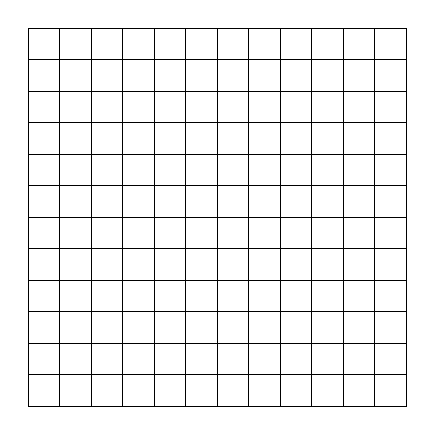
\begin{tikzpicture}[scale=0.4]
            \foreach \x in {0,1,2,...,12}
                {
                    \draw (\x,0)--(\x,12);
                }
            \foreach \y in {0,1,2,...,12}
                {
                    \draw (0,\y)--(12,\y);
                }
            \draw(0,0)--(12,0)--(12,12)--(0,12)--cycle;
        \end{tikzpicture}
        \hspace{1cm}
        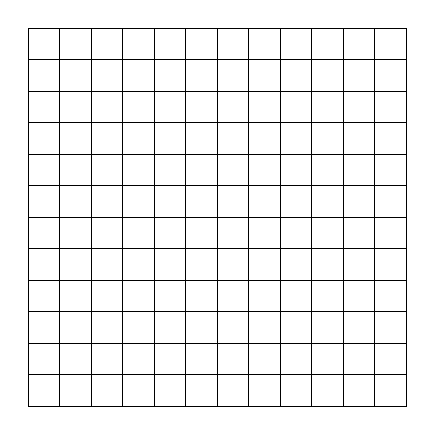
\begin{tikzpicture}[scale=0.4]
            \foreach \x in {0,1,2,...,12}
                {
                    \draw (\x,0)--(\x,12);
                }
            \foreach \y in {0,1,2,...,12}
                {
                    \draw (0,\y)--(12,\y);
                }
            \draw(0,0)--(12,0)--(12,12)--(0,12)--cycle;
        \end{tikzpicture}
    \end{figure}
    \item 仔细地画一个草图,说明如果按照平行四边形法则将$\bb{u}$与$\bb{v}$相加,然后让$(\bb{u}+\bb{v})$与$\bb{w}$相加,最终得到的将是一个以$(\bb{u}$、$\bb{v})$和$\bb{w}$为边线的平行六面体的对角线。
    \item 用文字和草图设计一个实验,说明力的叠加满足矢量加法运算法则。
    \item 若$\bb{u}\sim (2,-3,4)$,$\bb{v}\sim (1,0,1)$,计算$\bb{u}\cdot \bb{v}$的值与它们之间的夹角。
    \item 计算例题1.4中出现的矢量的$\mathrm{Proj}_u\bb{v}$和$\mathrm{Proj}_v\bb{u}$。
    \item 华盛顿特区大致位于北纬39°和西经77°,莫斯科特区大致位于北纬56°和东经38°。取地球的半径为4000英里(miles),计算出这两个城市之间的圆弧距离。
    
    提示:想象一下从地球中心到城市的矢量,并使用点积。
    \item 利用式\eqref{equ:1.11},在不引入笛卡尔坐标的前提下证明:矢量加法的分配律。
    
    提示:如果$\bb{a}$和$\bb{b}$是一个平行四边形的共端边,那么$2\left| \bb{a} \right|^2+2\left| \bb{b} \right|^2=\left| \bb{a}+\bb{b} \right|^2+\left| \bb{a}-\bb{b} \right|^2$。将式\eqref{equ:1.11}应用于$\bb{u}\cdot \left( \bb{v}+\bb{w} \right) $,并在结果表达式中设$\bb{v}+\bb{w}-\bb{u}=\left( \bb{v}-\frac{1}{2}\bb{u} \right) +\left( \bb{w}-\frac{1}{2}\bb{u} \right) =\bb{a}+\bb{b}$。
    \item Schwarz不等式
    \begin{equation}\label{equ:1.8*}
        \left| \bb{u}\cdot \bb{v} \right|\le \left| \bb{u} \right|\left| \bb{v} \right|\tag{*}
    \end{equation}
    是一个简单的几何定理的例子,它对于函数也有一个类似的有用结论:若函数$f$和$g$在区间$(a,b)$内平方可积,那么
    \begin{equation}\label{equ:1.8**}
         \left| \int_a^b{f\cdot g\mathrm{d}x} \right|\le \sqrt{\int_a^b{f^2\mathrm{d}x}}\sqrt{\int_a^b{g^2\mathrm{d}x}}\tag{**}
    \end{equation}
    \begin{enumerate}
        \item 用三种方法证明:式\eqref{equ:1.8*}:
            \begin{enumerate}[(i)]
                \item 利用式\eqref{equ:1.25}和定理
                \begin{equation*}
                    \left| \bb{u}\times \bb{v} \right|^2\ge 0
                \end{equation*}
                \item 利用定理:对于任意$x\in \mathbb{R} $二次多项式
                \begin{equation*}
                    p\left( x \right) =\left| \bb{u}+x\bb{v} \right|^2
                \end{equation*}
                非负。
                \item 利用式\eqref{equ:1.11}和欧式几何中的定理:三角形中,两边之差小于等于第三边。
            \end{enumerate}
        \item 利用与(i)和(ii)类似的方法证明:式\eqref{equ:1.8**}。
    \end{enumerate}
    \item 设$\bb{a}$、$\bb{b}$表示已知的三维矢量,而$\bb{x}$未知。不引入分量,证明:线性代数方程
    \begin{equation}\label{equ:1.9 *}
        \bb{x}+\bb{a}\times \bb{x}=\bb{b}\tag{*}
    \end{equation}
    的唯一解是
    \begin{equation*}
        \bb{x}=\frac{\bb{b}+\left( \bb{a}\cdot \bb{b} \right) \bb{a}+\bb{b}\times \bb{a}}{1+\bb{a}\cdot \bb{a}}
    \end{equation*}

    提示:设$\bb{x}=A\bb{a}+B\bb{b}+C\bb{a}\times \bb{b}$,然后求出系数$A,B,C$。为了证明:解的唯一性,可以设$\bb{y}$为方程\eqref{equ:1.9 *}的另一个解,然后证明:
    \begin{equation*}
        \bb{x}-\bb{y}+\bb{a}\times \left( \bb{x}-\bb{y} \right) =0
    \end{equation*}
    那么,你能从唯一性中总结出什么呢?
    \item 若$\bb{a}\sim (-2,1,0)$,$\bb{b}\sim (3,2,1)$,
    \begin{enumerate}
        \item 计算$\bb{a}\times \bb{b}$
        \item 写出$\bb{a}$、$\bb{b}$所确定的平面的方程。
    \end{enumerate}
    \item 给定点$P(x_0,y_0,z_0)$和平面
    \begin{equation}\label{equ:1.11*}
        \Pi :Ax+By+Cz=D\tag{*}
    \end{equation}
    利用以下方法推导从$P$到$\Pi $的(最短)距离公式:
    \begin{enumerate}
        \item 利用微积分,计算平面\eqref{equ:1.11*}上$(x-x_0)^2+(y-y_0)^2+(z-z_0)^2$的条件极小值
        \item 利用矢量方法构造$a$由$P$到$\Pi$且垂直于$\Pi$。
        
        提示:请回忆$\bb{N}\sim (A,B,C)$的含义。
    \end{enumerate}
    \item 若$\bb{u}\sim (1,-1,2),\bb{v}\sim (3,2,1),\bb{w}\sim (4,1,7)$,请计算
    \begin{enumerate}
        \item $\bb{uv}(\bb{w})$
        \item $\bb{vu}(\bb{w})$
        \item $\bb{wu}(\bb{u})$
    \end{enumerate}
    \item 证明:
    \begin{enumerate}
        \item $(\bb{uv})^{\mathrm{T}}=\bb{vu}$
        \item 对于任意矢量$\bb{a},\bb{b},\bb{c}$,$(\bb{a}\times\bb{b})\times \bb{c}=(\bb{ba}-\bb{ab})(\bb{c})$
    \end{enumerate}
    \item 利用微积分或是几何方法(这里用物理模型很方便)证明:由$\bb{u},\bb{v},\bb{w}$作为共端边的四面体的体积是$\frac{1}{6}\left| \left( \boldsymbol{u}\times \boldsymbol{v} \right) \cdot \boldsymbol{w} \right|$。
    \item 给出一个可信(尽管可能不甚严谨)的证明:,说明由$\bb{u},\bb{v}$作为共端边的平行四边形,在垂直于$\bb{w}$的平面上的投影面积为$\left| \left( \boldsymbol{u}\times \boldsymbol{v} \right) \cdot \overline{\boldsymbol{w}} \right|$。
    \item 证明:在三维空间中\label{exercise:1.16}
    \begin{equation*}
        \boldsymbol{u}=\boldsymbol{v}\Longleftrightarrow \boldsymbol{u}\times \boldsymbol{c}=\boldsymbol{v}\times \boldsymbol{c}\,\, ,\forall \boldsymbol{c}
    \end{equation*}
    \item 取$\bb{T}$为例题1.4中定义的矢量\label{exercise:1.17}
    \begin{enumerate}
        \item 若$\bb{v}\sim (v_x,v_y,v_z)$,填空:
        
        $\boldsymbol{Sv}=\frac{1}{2}\left( \boldsymbol{T}+\boldsymbol{T}^{\mathrm{T}} \right) \boldsymbol{v}\sim \left( \_\_,\_\_,\_\_ \right) $

        $\boldsymbol{Av}=\frac{1}{2}\left( \boldsymbol{T}-\boldsymbol{T}^{\mathrm{T}} \right) \boldsymbol{v}\sim \left( \_\_,\_\_,\_\_ \right) $
        \item 写出$\bb{S}$和$\bb{A}$的笛卡尔坐标矩阵。
        \item 写出矢量$\bb{\omega}$的笛卡尔坐标,使得$\bb{A}=\bb{\omega}\times$。
    \end{enumerate}
    \item 设$\bb{A}$表示任意三维反对称张量
    \begin{enumerate}
        \item 用笛卡尔坐标表示$\bb{A}$(注意,由于$\bb{A}=-\bb{A}^{\mathrm{T}}$,仅有三个分量是任意的),找出一个矢量$\bb{\omega }$使得
        \begin{equation*}
            \boldsymbol{Av}=\boldsymbol{\omega }\times \boldsymbol{v}\,\, ,\forall \boldsymbol{v}
        \end{equation*}
        \item 用练习\ref{exercise:1.16}的结果证明:$\bb{\omega }$唯一。$\omega $被称作$\bb{A}$的转轴,它在刚体动力学中很重要。见练习4.20。
        \item 证明:$\bb{v}\cdot \bb{Av}=0$吗,其中$\bb{v}$为任意$n$维矢量。
        \item 证明:$\bb{A\omega}=0$,并用练习1.\ref{exercise:1.17}(c)中得到的数值检验它。
    \end{enumerate}

    \begin{figure}[htbp]
        \centering
        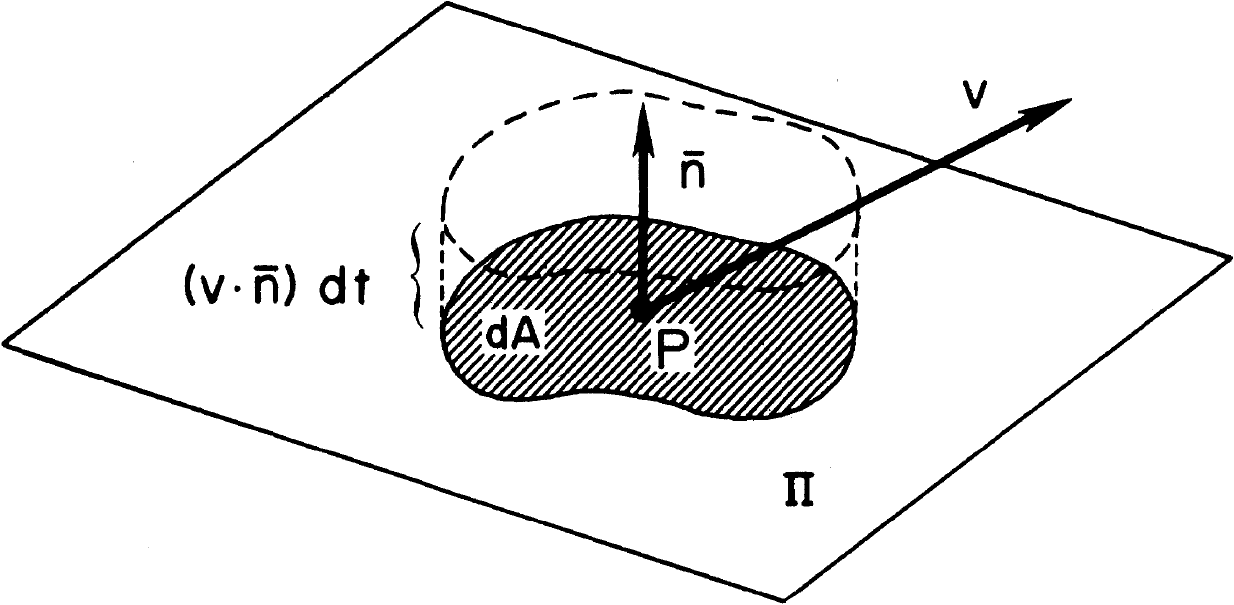
\includegraphics[width=0.65\textwidth]{./image/1.9.png}
        \caption{}
        \label{fig:1.9}
    \end{figure}

    \item 用$\rho $和$\bb{v}$分别表示$t$时刻空间中某点$P$处流体的密度和流速。若$\Pi $表示法线$n$过$P$点的平面,那么$t$时刻在$P$点处穿过$\Pi$的动量通量定义为$\rho \boldsymbol{v}\left( \boldsymbol{v}\cdot \widehat{\boldsymbol{n}} \right) =\rho \boldsymbol{vv}\left( \widehat{\boldsymbol{n}} \right) $。如图\ref{fig:1.9}所示,$\rho \boldsymbol{v}\left( \boldsymbol{v}\cdot \widehat{\boldsymbol{n}} \right) \mathrm{d}A\mathrm{d}t$表示$t$时刻$P$点处在$\mathrm{d}t$时间内穿过面元$\widehat{\boldsymbol{n}}\mathrm{d}A$的有向微元。$\rho \boldsymbol{vv}$被称作$t$时刻$P$点处动量流密度张量(或者叫它动量通量张量)。
    \begin{enumerate}
        \item 若$\bb{v}\sim (v_x,v_y,v_z)$,写出$\rho \boldsymbol{vv}$的笛卡尔坐标。
        \item 若给定时空点处$\bb{v}\sim (3,-1,2)$,$\rho =4$,写出穿过法矢为$\boldsymbol{n}\sim \left( -1,1,3 \right) $的平面的动量通量。
    \end{enumerate}

    \begin{figure}[htbp]
        \centering
        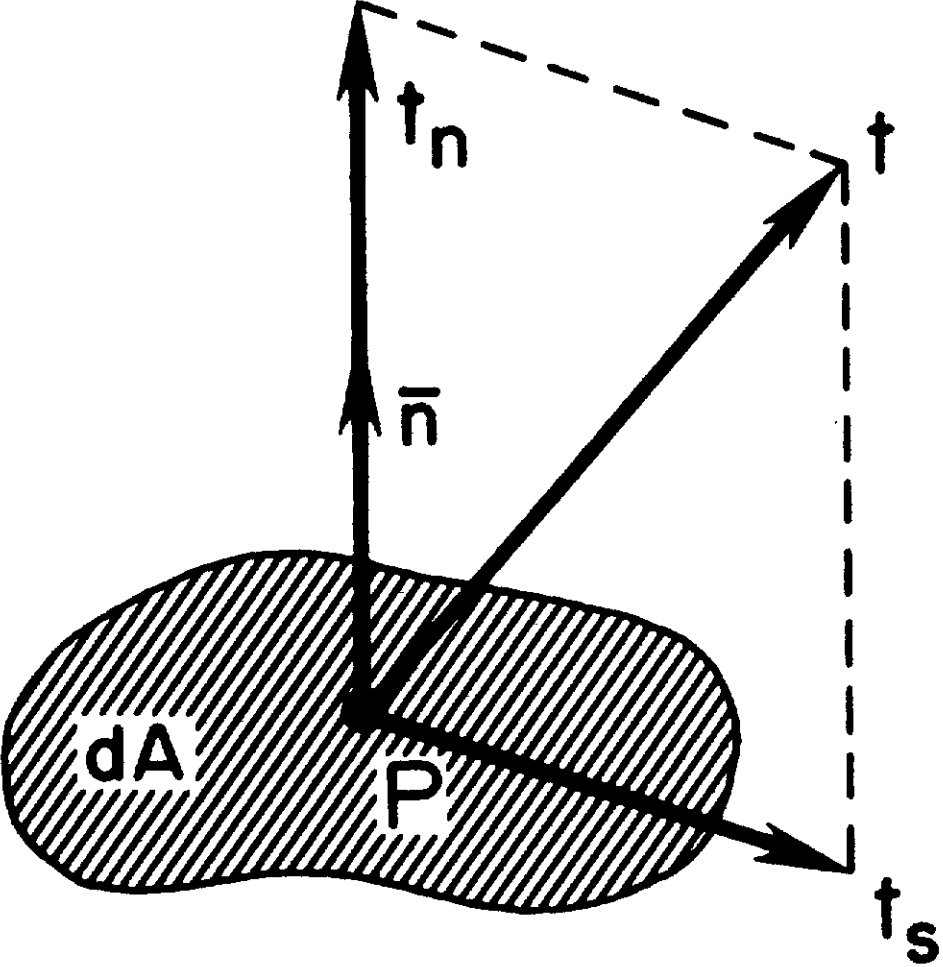
\includegraphics[width=0.35\textwidth]{./image/1.10.png}
        \caption{}
        \label{fig:1.10}
    \end{figure}

    \item 如图\ref{fig:1.10}所示,设$\widehat{\boldsymbol{n}}\mathrm{d}A$表示$t$时刻$P$点处连续介质(例如,流体或是固体)中的有向面元,设$\boldsymbol{t}\mathrm{d}A$表示材料施加于面元$\mathrm{d}A$的$\bb{n}$方向的力。$\bb{t}$被称作$t$时刻$P$点处$\widehat{\boldsymbol{n}}$方向的应力;$\boldsymbol{t}_n=\mathrm{Proj}_n\boldsymbol{t}$被称作法向应力,而$\boldsymbol{t}_s=\boldsymbol{t}-\boldsymbol{t}_n$被称作剪应力。通过考察以$P$点为中心的任意小四面体的瞬时运动方程,我们可以证明:$\boldsymbol{t}=\boldsymbol{T}\widehat{\boldsymbol{n}}$,其中$\boldsymbol{T}=\boldsymbol{T}^{\mathrm{T}}$为$t$时刻$P$点处的(柯西)应力张量\footnote{所有单位向量的集合不是线性向量空间(为什么?),因此它不是$\bb{T}$合适的定义域。然而,应力张量的定义和定义域可以用一种清晰的方式延拓,正如Noll所说,$\boldsymbol{T}\bf{0}=\bf{0},\boldsymbol{Tv}=\left| \boldsymbol{v} \right|\boldsymbol{T}\widehat{\boldsymbol{v}}\,\, ,\forall \boldsymbol{v}\ne \bf{0}$。}。若
    \begin{equation*}
        \boldsymbol{T}\sim \left[ \begin{matrix}
            1&		0&		0\\
            0&		3&		1\\
            0&		-1&		3\\
        \end{matrix} \right] 
    \end{equation*}
    并且$\bb{n}\sim (1,2,-1)$,计算法向应力以及剪应力。
    \item 主应力的方向定义为与单位矢量$\bb{x}$的方向相同,其满足$\bb{Tx}=\lambda\bb{x}$。注意,$\lambda\bb{x}$仅表示主应力,其剪应力在主方向上为零。确定$\lambda$所有可能的取值和$\bb{x}$的关联方向方向的问题被称作特征值问题。你可能已经在线性代数中看过这种问题。求出上一题中应力张量$\bb{T}$的特征值$\lambda$和关联方向$\bb{x}$。
    \item \begin{enumerate}
        \item 确定直积$\bb{uv},\bb{uw}$和$\bb{vw}$的笛卡尔坐标矩阵,其中$\bb{u,v}$和$\bb{w}$由练习1.12给出。
        \item 计算$\det(\bb{uv}),\det(\bb{uw})$和$\det(\bb{vw})$
        \item 证明:任意两个矢量直积的行列式等于零。
    \end{enumerate}
    \item 直积的迹被定义为
    \begin{equation*}
        \mathrm{tr}\left( \boldsymbol{uv} \right) =\boldsymbol{u}\cdot \boldsymbol{v}\,\, , \,\, \mathrm{tr}\left( \boldsymbol{uv}+\boldsymbol{wx} \right) =\mathrm{tr}\left( \boldsymbol{uv} \right) +\mathrm{tr}\left( \boldsymbol{wx} \right) 
    \end{equation*}
    根据定义和式\eqref{equ:1.46},计算$\tr \bb{T}$的笛卡尔坐标表达式。
    \item 张量$\bb{T}$的特征值,决定于单一参量$t$,可以由此定义
    \begin{equation}
        \dot{\boldsymbol{T}}\boldsymbol{a}=\left( \boldsymbol{Ta} \right) ^{\cdot}
    \end{equation}
    \begin{enumerate}
        \item 根据定义,$\bb{T}$将一个矢量转换成另一个矢量。证明:$\dot{T}$是线性的,也因此是一个二阶张量。
        \item 若$\bb{v}\sim (v_X,v_y,v_z)$,其中$\bb{v}$由$t$决定,并且$\bb{Tv}\sim ( -2t^2v_x+3t^2v_z , \cos \pi tv_z ,$$ v_x+2tv_y+\sqrt{1+t^2}v_z ) $,请填空:$\dot{\boldsymbol{T}}\boldsymbol{v}\sim \left( \_\_\_,\_\_\_,\_\_\_ \right) $
        \item 若$\bb{T}=\bb{xy}$,其中$\bb{x}$和$\bb{y}$是参数$t$的函数,$\dot{\bb{T}}$是?
        \item 如果给出$\bb{T}$的笛卡尔坐标,我们如何得到$\dot{\bb{T}}$?
    \end{enumerate}
    \item 两个二阶张量$\bb{S}$和$\bb{T}$的分量或点积也是一个二阶张量,可记作$\bb{S}\cdot \bb{T}$,其定义为
    \begin{equation*}
        \boldsymbol{S}\cdot \boldsymbol{Tv}=\boldsymbol{S}\left( \boldsymbol{Tv} \right) \,\, \forall \,\,\boldsymbol{v}
    \end{equation*}
    \begin{enumerate}
        \item 若$\bb{S}=\bb{wx}$,$\bb{T}=\bb{yz}$,求$\bb{S}\cdot \bb{T}$。
        \item 若$\bb{S}$和$\bb{T}$是关于$t$的可微函数,证明:
        \begin{equation}
            \left( \boldsymbol{S}\cdot \boldsymbol{T} \right) ^{\cdot}=\boldsymbol{S}\cdot \dot{\boldsymbol{T}}+\dot{\boldsymbol{S}}\cdot \boldsymbol{T}
        \end{equation}
    \end{enumerate}
    \item 参考练习1.18a并利用式\eqref{equ:1.22},证明:
    \begin{equation}\label{equ:1.49}
        \left( \bb{\omega } \times \right) ^2=\bb{\omega } \times \left( \bb{\omega } \times \right) =\boldsymbol{A}^2=\bb{\omega } \bb{\omega } -\left( \bb{\omega } \cdot \bb{\omega } \right) \bb{1}
    \end{equation}
    同时由此可以得到
    \begin{equation*}
        \left| \boldsymbol{\omega } \right|^2=-\frac{1}{2}\tr \boldsymbol{A}^2
    \end{equation*}
    \item 二阶张量的逆。如果函数$f$满足$f\left( x_1 \right) =f\left( x_2 \right) \Rightarrow x_1=x_2$,那么我们称其为单射。此时,对于任意$x$属于$f$的定义域,函数$f$有唯一的反函数$f^{-1}$,其满足$f^{-1}\left( f\left( x \right) \right) =x$。进一步地,对于任意$y$属于$f$的值域,$f\left( f^{-1}\left( y \right) \right) =y$。若$\bb{T}$是二阶张量,那么由张量的线性性可知$\boldsymbol{Tv}_1=\boldsymbol{Tv}_2$蕴含$\boldsymbol{T}\left( \boldsymbol{v}_1-\boldsymbol{v}_2 \right) =0$。若$\bb{T}$是非奇异的,那么反过来,这意味着$\bb{v}_1=\bb{v}_2$。因此,$\bb{T}$有唯一的逆$\bb{T}^{-1}$使得
    \begin{equation}
        \begin{aligned}
            \boldsymbol{T}^{-1}\cdot \boldsymbol{Tv}&=\boldsymbol{v}\,\, ,  \forall \boldsymbol{v}\\
            \boldsymbol{T}\cdot \boldsymbol{T}^{-1}\boldsymbol{w}&=\boldsymbol{w}\,\, ,  \forall \boldsymbol{w}
        \end{aligned}
    \end{equation}
    \begin{enumerate}
        \item 证明:$\bb{T}^{-1}$是线性的(并且因此是一个二阶张量)
        \item 证明:$\left( \boldsymbol{T}^{-1} \right) ^{\mathrm{T}}=\left( \boldsymbol{T}^{\mathrm{T}} \right) ^{-1}$。
        \item 证明:例题1.4中的张量是非奇异的。
        \item 若$\boldsymbol{w}\sim \left( w_x,w_y,w_z \right) $而$\bb{T}$是例题1.4中的张量,填空:$\boldsymbol{T}^{-1}\boldsymbol{w}\sim \left( \_\_,\_\_,\_\_ \right) $。
        
        提示:设$\boldsymbol{T}^{-1}\boldsymbol{w}\sim \left( a,b,c \right) $,并注意$\bb{T}$作用于$\bb{T}^{-1}\bb{w}$必须等于$\bb{w}$。
    \end{enumerate}
    \item 我们说二阶张量$\bb{T}$是正定的,如果
    \begin{equation*}
        \begin{matrix}
            \boldsymbol{x}\cdot \boldsymbol{Tx}>0&		\forall \boldsymbol{x}\ne \bf{0}
        \end{matrix}
    \end{equation*}
    \begin{enumerate}
        \item 证明:若$\bb{T}$是正定的,那么$T$所有的特征值都是正的。
        \item 证明:若$\bb{T}$是非奇异的,那么$\boldsymbol{T}^{\mathrm{T}}\cdot \boldsymbol{T}$是正定的。
    \end{enumerate}
\end{exercise}